% Chapte 8 
\chapter{Interactive and non-Interactive Advertisement field study} % Main chapter title

\label{Chapter8} % For referencing the chapter elsewhere, use \ref{Chapter1} 
\newpage




\section{Introduction}



\hilight{Talk more general on advertisement and other displays }

Evaluating high-fidelity prototypes of advertisement provided several of feedbacks to refine them for the final evaluation on the field, the study focuses on conducting a \emph{summative study} \cite{summative} ``\emph{is used to evaluate how well the design meets the usability requirements}'' it is to make some final decisions on the prototype in this case Interactive advertisement with large number of participants on the field. There have been many kinds of these tests in lab and also in field, as Beyer, G \cite{CylindricalScreen} in which the user behavior and user experience was compared between flat and cylindrical displays, and Müller, J \cite{LookingGlass} did a study on how passers-by notice interactivity of public displays, the studies were done in both lab and field environments, Another study conducted by Anthony Tang \cite{Bystanders} that focused on consequences of the design choices with respect to encouraging \emph{bystanders} to interact with the public displays, and classified \emph{bystanders} who may never engage with the displays but contribute to interaction at some level.
Junko Ichino \cite{DisplayAngleEffect} researched on how different display angles could impact social behaviors of people around displays and also in one of his another paper \cite{DisplayAngleEffect2} investigated on User's cognition and subjective responses in relation to different display angles.

Audience Behavior is an important research question in most of the public display evaluations; audience behavior is how a person or user(s) react around a situated display, for example the (1) \emph{honeypot} \cite{EnticingPeople} that is the effect that people who are already involved in interaction with display attract other people around, it is also called ``\emph{sociable buzz}'' by the author, in public displays this effect can even create multiple rows of people interacting \cite{LookingGlass}. Another audience behavior is (2) \emph{landing effect} \cite{LookingGlass}, where the passers-by realize the interactivity of the display after they passed the display and they tend to walk back for confirmation or for interaction. Another audience behavior is (3) \emph {sweet spot} \cite{CylindricalScreen} where is a location that most people stand in relation to the display. At some occasions individuals do not feel comfortable by the presence of other people or situated displays and they tend avoid \cite{DesignSpace} and researches have been done to investigate spaces around display and on how to design a shared space for displays \cite{chained_displays}.

Effectiveness is another important area for public display evaluation, which is defined by many factors (also discussed on chapter 3) like (1) Number of passers-by \cite{glancingcount, digitalSignage}, (2) among passers-by how many glanced \cite{glancingcount, When_display, display_blindness} to it, (3) how many started interacting \cite{LookingGlass, glancingcount} and (4) how long passers-by were engaged with display.


This study also focuses on user behaviors (landing effect and honeypot effects) attractiveness, effectiveness of Non-interactive and interactive advertisement application and compares them among each other. The field study was executed in Weimar tourist Information Center at (Weimar Markt 10) which is one of important location for many tourists who visit Weimar. This location was chosen by Bauhaus-Spaziergang program personals that are providing tours for new visitors in Weimar. Bauhaus-Spaziergang does advertisement as brochure at this location. The location was reserved for our new advertisement starting from 1st February for three weeks.  

Two different Interactions and one non-Interactive Advertisement were made as described in previous chapters, the first one was body interaction where passers-by can interact using his/her own body movement in the physical space and influence advertisement element, and the second was mobile interaction, where users by opening the advertisement web application in their smartphone can interact with advertisement and the third is a non-interactive advertisement where the interface and elements are completely similar but are not influence by people around, the elements change based on time-based random sequence.



\section{Interactive Advertisement}

The interactive advertisement was originally designed as a three distinctive phases.


\begin{enumerate}

\item \textbf{Attraction / Motivation phases:}\\ 
This phase is the first interface for the advertisement, the passerby silhouettes are being projected on the screen and in this interface Call-to-action is implemented to motivate passers-by to start interacting with the screen.
Call-to-action techniques were different for mobile and body interactive system.

\item \textbf{Interaction phase:} \\
This phase allows participants to actively influence the advertisement elements, which were highlighted regions of Bauhaus in Weimar, the participant could explore those regions just by reaching to them, a picture of the area with a short description would appear for three seconds and then fade out. This phase is constraint with time and will automatically be over with in 40 seconds and would switch to the last phase called ad video phase.

\item \textbf{Advertisement video phase:} \\
This phase only shows a 20 second non-interactive Bauhaus-spaziergang Ad video and whenever the video is over it will switch back to the initial phase.

\end{enumerate}

\subsection{Body Interactive}

The body interactive advertisement has the ability to detect up to seven people at a time and project their silhouette in the screen each with different colors, the Call-to-Action feature asks viewers to come near to the screen to start the interaction, when the interaction starts participants are given a short instruction on how to play the system, participants should walk physically in front of the screen in order to move the silhouette on the map to explore the regions. The interaction finishes if all the regions are explored or the 40 second time gets over and the Ad video is shown.


\begin{figure}[H]
    \centering
    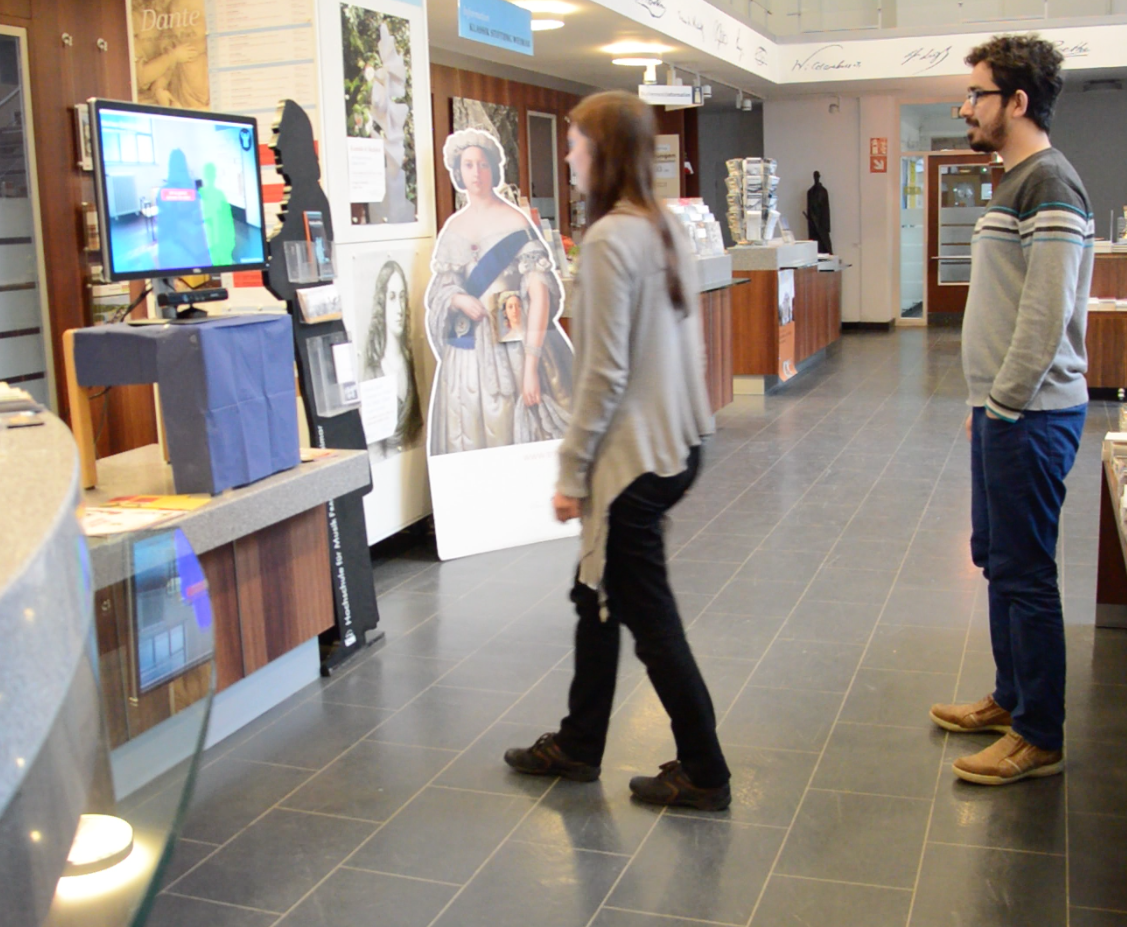
\includegraphics[width=110mm,height=70mm]{Figures/8/body_motivation}%
    \caption{Two persons are standing far from the screen, and their colored silhouettes are shown, the girl is getting closer to the screen to start the interaction.}%
    \label{fig:bodymotivationsystem}%
\end{figure}

\begin{figure}[H]
    \centering
    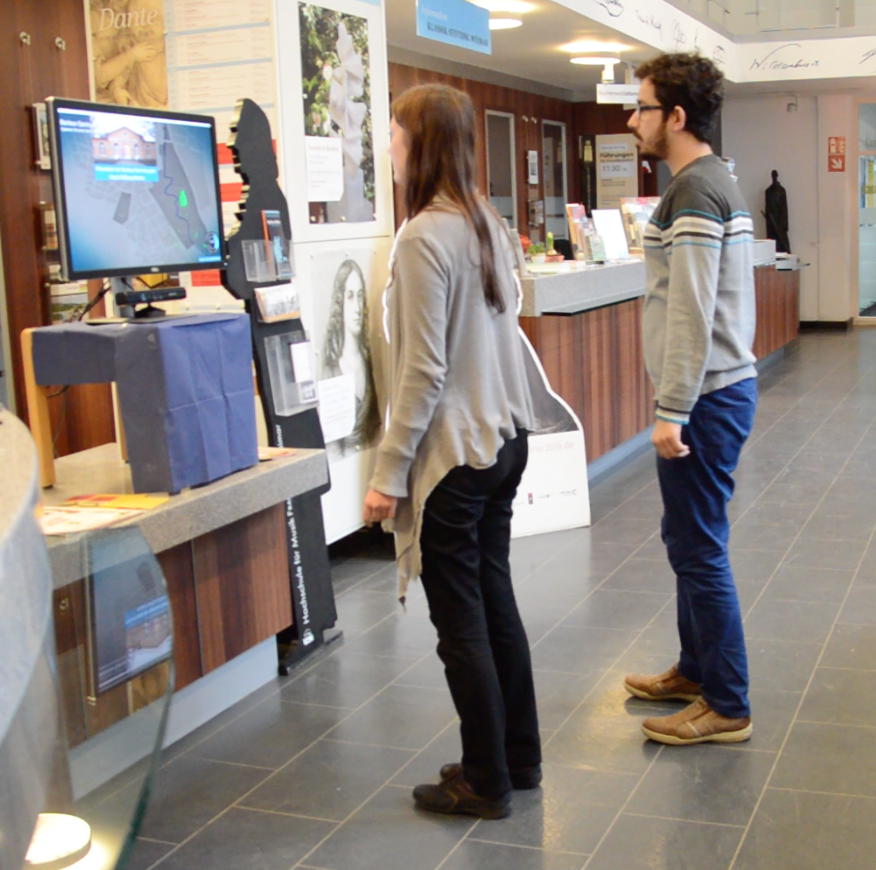
\includegraphics[width=110mm,height=70mm]{Figures/8/body_interaction}%
    \caption{Both are in interaction phase, as you can see the girl has explored one location and a picture is shown}%
    \label{fig:bodyinteractionsystem}%
\end{figure}

\subsection{Mobile Interactive}
As you already got the idea that this technique works with smart phone, the system also shows partially passers-by silhouette for attracting attention, but the Call-to-Action is done through using a mobile phone, the screen gives instruction on how to access the system. Passerby should connect to the wireless local area network and browse the controller website from their phone, and the control opens in their phone to use navigate to different regions on the map to explore interest locations. The interaction is also constraint to 40 second time and after that the Ad video is shown.


\begin{figure}[H]
    \centering
    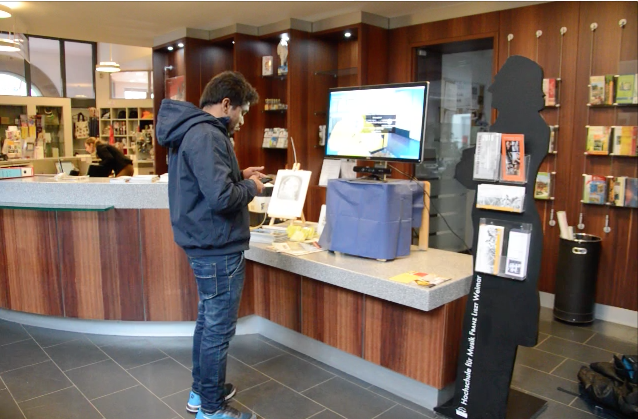
\includegraphics[width=110mm,height=70mm]{Figures/8/mobile_motivation}%
    \caption{The person is connecting to the advertisement web controller using his phone.}%
    \label{fig:mobilemotivationsystem}%
\end{figure}


\section{Non-Interactive Advertisement}
This technique is also composed of the same three phases but each of them is triggered without the influence of people around, we call it auto active advertisement too. The first phase shows only the screen with the Bauhaus-spaziergang title and has no Call-to-Action feature and after few seconds switches to the second phase, in second phase the locations are automatically explored in random sequence each time and has the same expiration time (40 seconds) as others and after that the same ad video is shown and switches back to the first mode. The entire cycle of the phases is around 60 seconds which is almost similar to the other two interactive advertisement.


\begin{figure}[H]
    \centering
    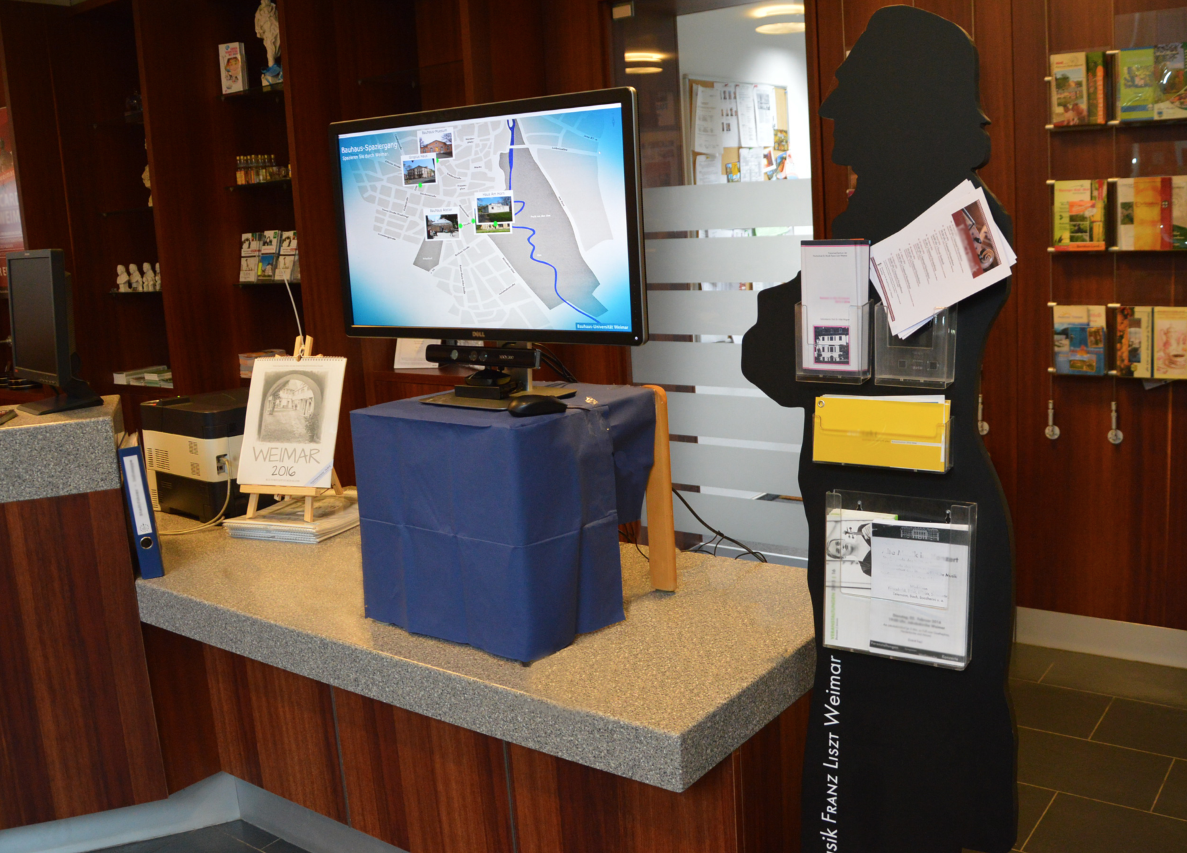
\includegraphics[width=110mm,height=70mm]{Figures/8/non_inter_screen}%
    \caption{The screen is automatically exploring locations on the map}%
    \label{fig:non-inteactivescreen}%
\end{figure}



\section{Research questions}
\begin{enumerate}

\item	For which of the three conditions (body, mobile and non-interactive advertisements) passers-by 

\begin{enumerate}
\item	Are more attracted toward?
\item	Perform Honeypot and Landing effects?
\item	Are engaged with the screen?
\item	Watch the remaining advertisement video after interaction?
\end{enumerate}

\item	How many people remember advertisement?
\item	What are passers-by feedback about the advertisement techniques?
\item	What are the difference between effectiveness and audience behavior for Interactive and Non-interactive advertisement?

\end{enumerate}




\section{Design study}


\subsection{Location}
The screen was installed in Weimar Tourist Information center. This center is one of the famouse tourist information in Weimar where alot of tourists visit. Most importantly this location was chosen because our target audience (tourists) mainly elders visit.

\begin{figure}[H]
    \centering
    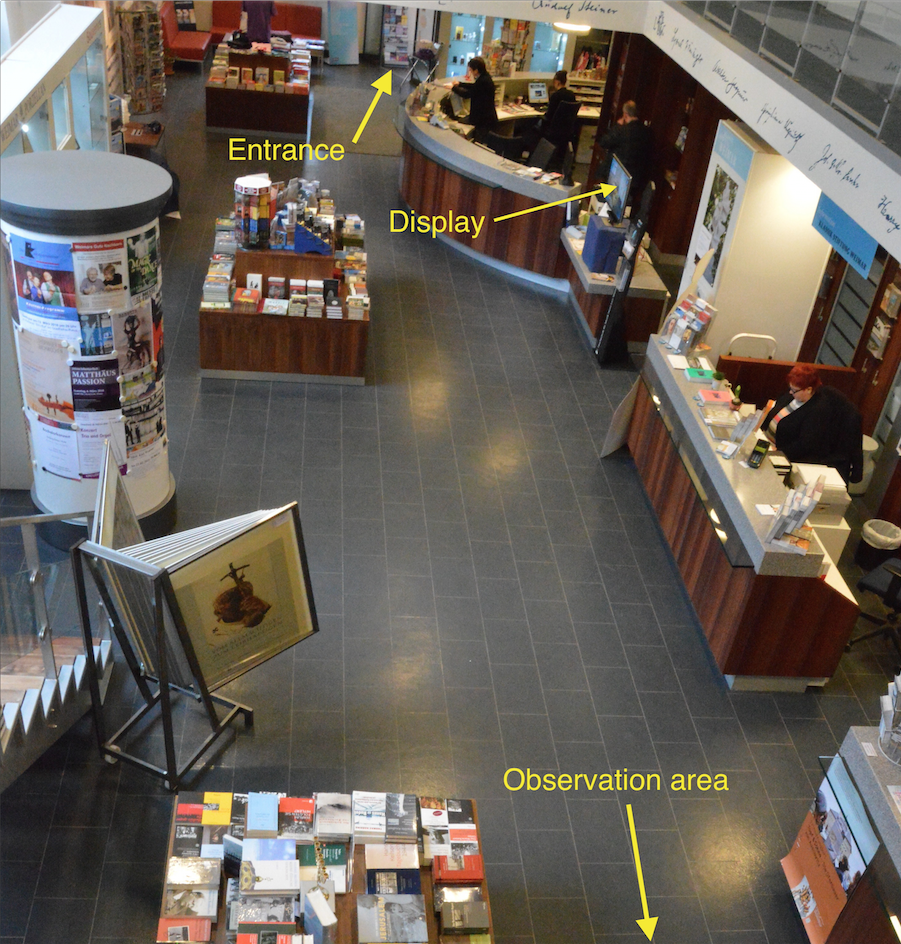
\includegraphics[width=110mm,height=90mm]{Figures/8/tourist_info}%
    \caption{Weimar Tourist Information Center Top-view picture, The locations are marked with yellow arrows.}%
    \label{fig:Tourist_info_center}%
\end{figure}


\subsection{Duration}
Each type of advertisement technique were installed for five days in the following three weeks.

\begin{table}[H]
\caption{Week sequence}
\label{tab:advertisementWeeks}
\centering
\begin{tabular}{l c c c }
\toprule
\tabhead{Advertisement} & \tabhead{1st Week} & \tabhead{2nd Week} & \tabhead{ 3rd Week} \\
\midrule
\textbf{Non-Interactive}     &   X    &         &     \\
\textbf{Body Interactive}     &        &    X    &    \\
\textbf{Mobile Interactive}  &        &         &   X   \\
\bottomrule\\
\end{tabular}
\end{table}



\subsection{Internal Validity}
To be confident that the change in the weeks would not effect the findings, 
extra effort was done to make all the week environmental conditions the same as much as possible. The screen was installed in the same location, had the same screen brightness, height and also the surroundings of the screen were not altered, we asked the responsible person in tourist information center not to change anything in the surrounding. The luck was also with us that almost the weather conditions were the same too, but the only thing we could not control was the number of passerby; The flow of passers-by were also be nearly the same.


\subsection{Participants}
The participants were the ones who pass by the screen, none of the participants were informed about this study nor any notes were put at the entrance. Roughly \%60 of the participants were elder aged between 30-60, \%25 were young and the rest \%15 were children.


\subsection{Data gathering}
Several types of data from different aspects were gathered for each individual week to be able for analyzing and also be able to answer new arising questions after the onsite evaluation, the bellow types of data were gathered.


\begin{enumerate}
\item \textbf{On-Site Observation} \\
Observation periods were arranged in two different time slots per day, the first time slot was from 10:00 – 12:00 and the second was from 14:00 – 16:00, except for Saturday and Sunday where the tourist information center was open only until 14:00, then the observation period was from 10:00-12:00 and 13:00-14:00. During these two time slots the bellow observations were made and to remove the effects of specific time order,the orders were counterbalanced.

\begin{enumerate}
\item \textbf{Attention Level measurement} \\
Attention level is how much a person gives attention to the display, which consist of number of glances and number of ignores and how much long a person is standing infront of the display.At the beginning gaze-tracking method was considered for accurate measurement of attention level, a very impressive work have been done from Intraface \cite{Intraface} that can not only detect glances but also human emotions at the time, but because of high flow rate that method was not used and instead the glance counting which was proposed by \cite{glancingcount} that has formalized a ranking system from which  glance is considered if a person reacts to the display by turning his/her head toward it that last less than 3 seconds.

One hour attention level counting for each time slot was conducted, in which the observer was writing the number of people passing by and how many of them glanced and ignored the screen.see the glance counting sheet in Appendix: \ref{AppendixA}.1

\item \textbf{Passerby behavior and Interviews} \\
During one hour per time slot per day the passerby behavior were observed like how they approach to the screen, how do they react, what path the passerby take and what are they looking for and even how they ignore the display and after they are done with the screen engagement a very short interview was taken from them. 

\end{enumerate}


\item \textbf{System Logs} \\
The Advertisement application can generate the bellow logs.
\begin{enumerate}

\item	\textbf{Non-Interaction application} \\
Only duration(seconds) spent in front of the display is logged for each individual person.

\item	\textbf{Interaction application}\\
For this type the system can detect

\begin{itemize}
\item	Time user joins.
\item	Interaction completion time.
\item	Number of tasks (locations) explored.
\item	Whole duration spent(sec).
\item	If the user has seen advertisement or not.
\end{itemize}

\end{enumerate}

\item \textbf{Interviews} \\
Interviews were taken from the passerby that had some sort of engagement with the display like for non-interactive advertisement the people were interviewed that they stood for a while and saw the advertisement and for the interactive advertisement the people were interviewed that interacted or tried to interact with the system.
A leaflet, that describes the thesis goal and interview consent form was handed to the participants and after signature the interview was conducted. All the interviews were audio recorded and later transcribed for analysis, all interviews took in average 4 minutes, the reason we took short interviews was that most of the people were tourists and had little time to stay and even some of them rejected interview because of shortage of time.
Each week there were some variation in the questions dependent to the type of advertisement.  See appendix \ref{AppendixD}.1


\item \textbf{Colored-image recording} \\
Colored-image recording from Kinect camera was done during entire three weeks for non-interactive and interactive advertisement for many reasons.

\begin{itemize}
\item Match the log data with the video data for accuracy.
\item Measure the number of Honeypot effects and landing effects.
\item Observe passerby behavior in detail.
\end{itemize}

Because of limited space and processing power, the actual depth information (x,y,z) for individual points was not stored but a 2D colored image was taken per second and after the image recording was done, in lab another post processing script was applied to integrate a static background using Adobe Photoshop application. To match the data logs and the image frames each image name consisted the date and time as (10.12.43.21.png).


\begin{figure}[H]
    \centering
    \begin{subfigure}[H]{0.45\textwidth}
        \centering
        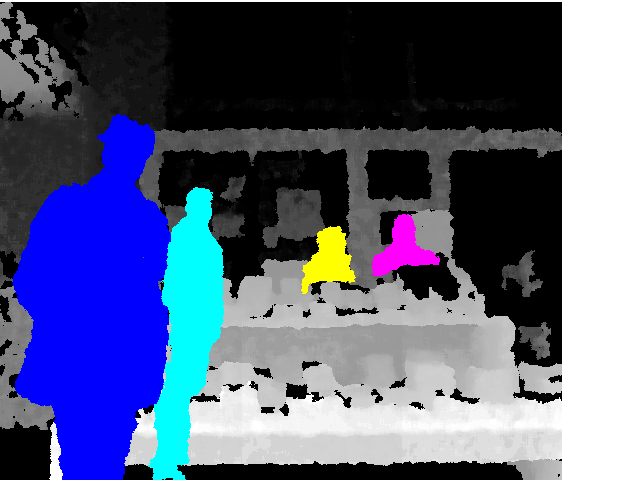
\includegraphics[width=\textwidth,height=4cm]{Figures/8/d1}
        \caption{}
        \label{fig:d1}
    \end{subfigure}
    \hfill
    \begin{subfigure}[H]{0.45\textwidth}
        \centering
        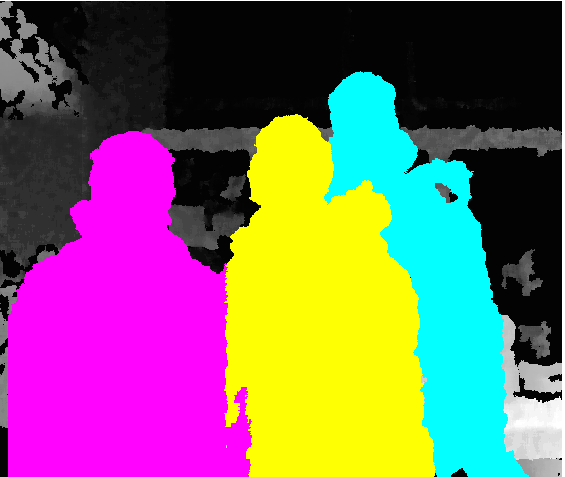
\includegraphics[width=\textwidth,height=4cm]{Figures/8/d2}
        \caption{}
        \label{fig:d2}
    \end{subfigure}
    \caption{Depth recording examples}
    \label{fig:DepthRecordedImages}
\end{figure}




\end{enumerate}

Other pictures were also taken using mobile phone from the scene, verbal permission were taken before the photographing them.


\newpage
\section{Data Analysing}

 
\subsection {Glance counts} 
The glance counts were transformed from paper to spreadsheet in which number of glances and ignores were recorded individually and then combined from which mean value and percentages are extracted. \hilight{fix appendix}see Appendix \ref{AppendixD}.2, \ref{AppendixD}.3 and \ref{AppendixD}.4 for each week.

\subsection {Interviews} 
All the interviews were transcribed and color coded from which interesting categories had emerged, each code is separately discussed in the finding section, To see color coded diagram see Appendix \ref{AppendixD}.5, \ref{AppendixD}.6 and \ref{AppendixD}.7 for each week. \hilight{fix appendix}


\subsection {Display Engagement phases and time} 
Log files along depth images were seen and compared to have accurate values for each engagement phases and the whole interaction phases. depth frames were manually frame-by-frame analysed and the logs were cleared from any possible mistakes.

\subsection {Honeypot and landing effects}
These two effects were observed mainly from the depth frames and also partially from onsite observation.

\subsection {Other observations}
The observations were done onsite, the observer wrote down any important event happened at that moment, These notes also include observer own point of view of understanding the scenario during the entire day and week. Most of the notes have time stamp. See Appendix \ref{AppendixD}.8, \ref{AppendixD}.9, and \ref{AppendixD}.11.\\
The depth recordings were also observed frame-by-frame to see anything that was missed when the observer was not present at the center. Different behaviors are extracted from the observation, which you will find in findings.



\newpage
\section{Findings}


\subsection{Non-Interactive findings}



\begin{enumerate}

\item \textbf{Attention Level measurements} 
The number of glances and ignores were measured for the five consecutive days as shown bellow, each day (bar) has less than half number of glances compared to number of ignores and in total the average glance is \%25, which corresponds to (1/4) portion of passers-by.


\begin{figure}[H]
    \centering
    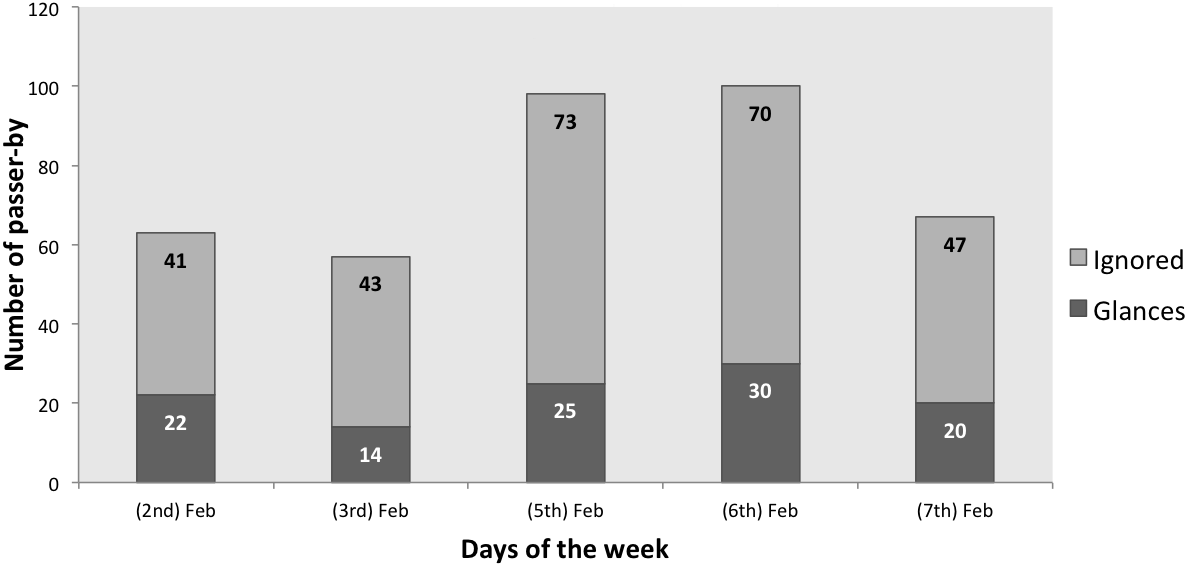
\includegraphics[width=110mm,height=55mm]{Figures/8/non_inter_findings/Non_Inter_chart}%
    \caption{Non-interactive attention level chart}%
    \label{fig:Nonattentionlevelchart}%
\end{figure}


\begin{figure}[H]
    \centering
    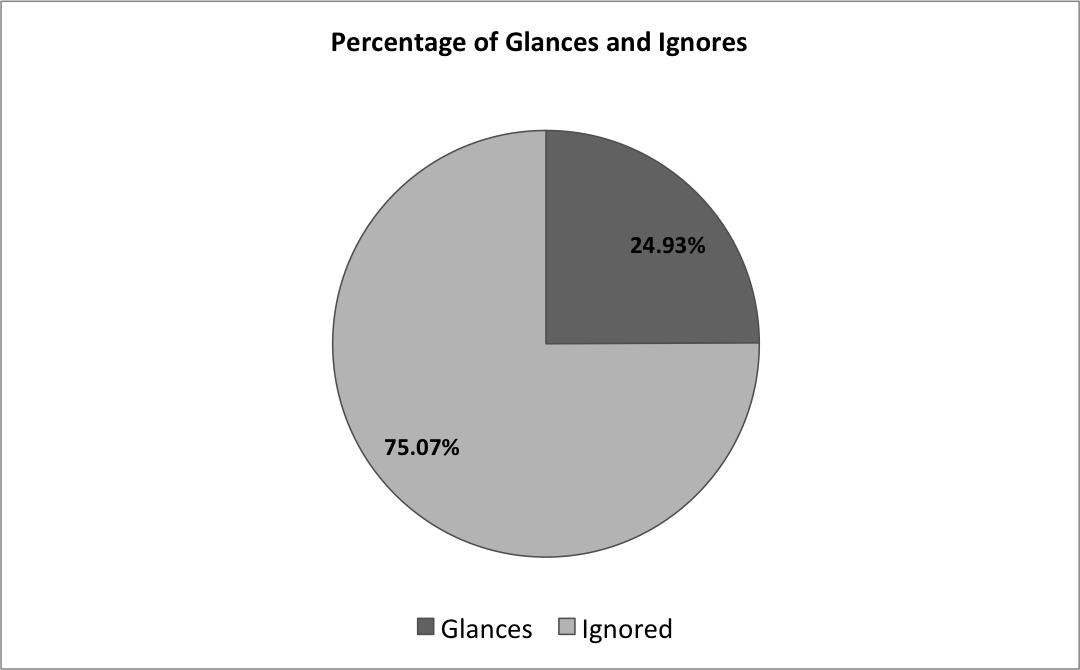
\includegraphics[width=110mm,height=55mm]{Figures/8/non_inter_findings/non_inter_percentage}
    \caption{Non-interactive Attention level percentage}%
    \label{fig:Nonattentionlevelpercentage}%
\end{figure}



\item \textbf{Engagement Time} \\
Not all people would take time to see the advertisement, some participants took very little time like 4-5 seconds and some also saw the ad for about 100 seconds which is almost twice of the advertisement time, so dependent to the interest people were engaged in different durations and in average it took about 34 seconds to be engaged.


\item \textbf{Passers-by and Engagement}
Counting the entire passers-by was a challenge and there was not accurate automated method to do therefor each day’s recordings were watched and the numbers of passers-by were counted manually, this intense work was carried out with a number of computer science students who voluntarily participated.  
And out of those passers-by the people who watched the screen for more than 5 seconds were flagged as an engaged passer-by.


\begin{figure}[H]
    \centering
    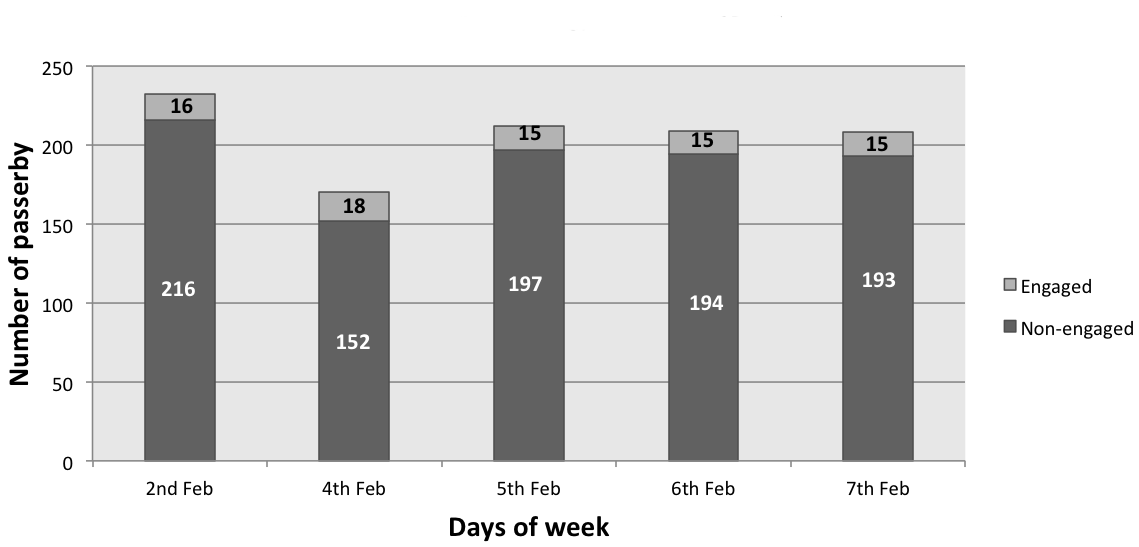
\includegraphics[width=110mm,height=60mm]{Figures/8/non_inter_findings/non_inter_engage_day}
    \caption{Non-interaction Number of engaged and Non-engaged passers-by}%
    \label{fig:Nonengagedandengagedby}%
\end{figure}

\begin{figure}[H]
    \centering
    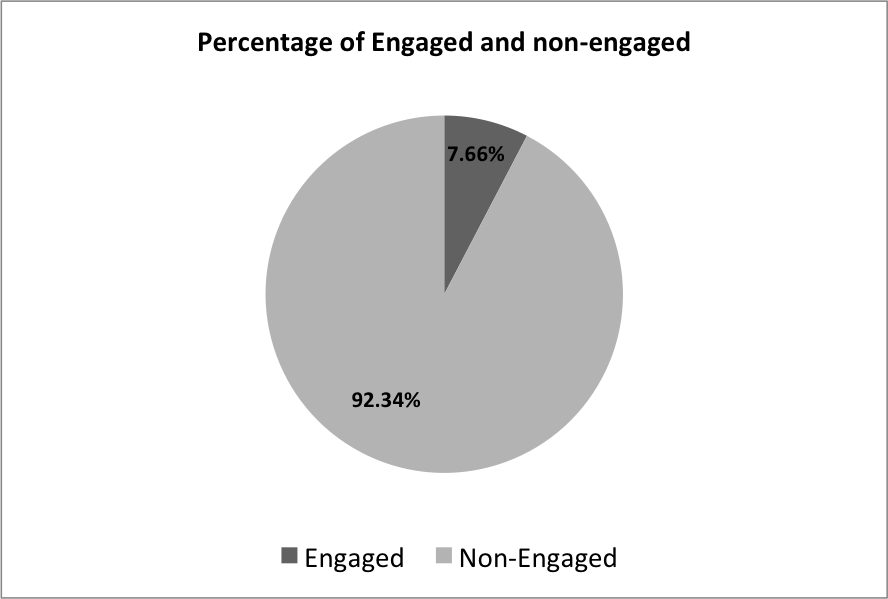
\includegraphics[width=110mm,height=60mm]{Figures/8/non_inter_findings/non_eng_percentage}
    \caption{Non-Interactive Percentage of engaged and passerby}%
    \label{fig:Nonengagedpasserbypercentage}%
\end{figure}


As can be seen in above chart it shows the number of passers who were engaged and number of passers-by who did was not engaged. The chart shows very few engaged people for each day and as an average \%7.66 of the whole population are engaged in 5 days.

\end{enumerate}


\newpage
\begin{enumerate}
\setcounter{enumi}{3}
\item \textbf{Landing and Honeypot effects} \\
\end{enumerate}

%\hilight{there is no honeypot or landing in non-interactive}
The bellow shows the frequencies of both effect for each day.


\begin{wrapfigure}{r}{0.4\textwidth}
  \vspace{-20pt}
  \begin{center}
    \includegraphics[width=0.30\textwidth,height=60mm]{figures/8/non_inter_findings/effects/landing}
  \end{center}
  \vspace{-20pt}
  \caption{Landing effect}
  \vspace{-10pt}
\end{wrapfigure}
The effects like honeypot or landing effects can not be defined in non-interactive displays but still similar incidents are seen. \\
In non-interactive the silhouette is not projected and the passers-by do not see theirselves in the screen but still for some other reasons (\hilight{define why}) turn back. As in the figure in the right (A) a person passes-by the display (B) then he notices something and he stops (C) He turns back toward display and (D) comes near to the screen. \\


\begin{wrapfigure}{r}{0.4\textwidth}
  \vspace{-20pt}
  \begin{center}
    \includegraphics[width=0.30\textwidth,height=60mm]{figures/8/non_inter_findings/effects/honeypot}
  \end{center}
  \vspace{-20pt}
  \caption{Honeypot effect}
  \vspace{-10pt}
\end{wrapfigure}
In picture (A) a lady is standing in front of the monitor and reading the content and after a while in picture (B) another person is approaching the monitor to see what is happening and immediately another person in picture (C, D) was also attracted to come close and see what is going on. 
The honeypot effect in non-interactive could be due to that a friend is watching the screen and another friend of him / her is attracted to the screen or just has another intension like to talk to or call him. The scenarios seemed to be very personal and during the observation not other than friends were attracted to see the screen.


\begin{table}[H]
\caption{Landing and honeypot effects}
\label{tab:landingandhonypot}
\centering
\begin{tabular}{| l | c | c |}
\toprule
\tabhead{Days} & \tabhead{Landing effect} & \tabhead{Honeypot effect} \\
\midrule
\textbf{2nd Feb}  & 1 &  1 \\
\textbf{4th Feb}  & 0 &  1 \\
\textbf{5th Feb}  & 2 &  3 \\
\textbf{6th Feb}  & 0 &  3 \\
\textbf{7th Feb}  & 1 &  1 \\
\bottomrule
\end{tabular}
\end{table}

\begin{enumerate}
\item \textbf{Interview} 
\begin{enumerate}
\item Likes \\
Many things from the advertisement were interesting, like the concept of map and the design. As one stated that, ``\emph{I find the idea good, it is nice to see the pictures of the places on the map}'', ``\emph{it is very nice idea because it will be remembered and when I go to the city I will remember}''

\item Dislikes \\
Most of the respondents complained on the speed of the advertisement that how fast the image changes as one said ``\emph{But the pictures were changing very fast}'' other said, ``\emph{advertisement is a little fast}'' They mentioned that why speed is an issue as stating, ``\emph{we wanted to see the map}'', ``\emph{ Could not read the text}''. Many things were disliked by some of the respondents like the advertisement theme, one said, ``\emph{It did not have Bauhaus Theme, the color and that design}'' One respondent also disliked the blinking points.

\item  Participation \\
Respondents mentioned the same excuses that were given at body interactive advertisement, one said, ``\emph{I will join if I am free}'', other said, ``\emph{I have no time}'', or ``\emph{if the weather is good}''. 

\item  Advertisement recall
People could recall the ad, as one mentioned, ``\emph{It is for a tour of Bauhaus in Weimar}'' other said, ``\emph{People can visit the city}'' and some mentioned directly the name of the program ``\emph{Bauhaus-Spaziergang}''.

\item Recommendations \\
There were many recommendations proposed by the responders, which was on content, speed, design.Content related recommendations was that one said, ``\emph{If the prices are mentioned it would be good so that they can decide if they want to take it or not}'' other said on timing, ``\emph{how long does this tour take so people arrange their}''. Another mentioned on speed like ``\emph{it must be little slow}''.

\end{enumerate}


\item \textbf{Note taking} \\
Note taking helped to analyze the environment and behavior of people around the display.
During the non-interactive technique week, the surrounding of display was very quite and very little people would come and read, individual’s would come at beginning first to read and then later if there was a friend would also join. In normal circumstances if there was a couple coming inside tourist information center one of them would ask question from the help disk and the other person would see around the posters and other things.  There was an interactive object in front of the display on the table, which many people tried to play.

See appendix  \ref{AppendixD}.8
\hilight{fix this appendix}

\end{enumerate}

\newpage
\begin{enumerate}
\setcounter{enumi}{6}
\item \textbf{Other audience behaviors}
\end{enumerate}

The behavior toward non-interactive during the 5 days observation seemed to be very calm and passive, passers-by selectively came to watch the screen there was no curiosity nor attractiveness that had driven their attention. It was thread as a source of information and whenever they approach the screen the participants would normally stand for a very short time and after looking for 1-2 pop-up pictures on the screen they would leave, except for participants that was looking for some events that stood for the complete duration of the advertisement. 

\begin{itemize}

\item Display negligence  \\
At most of the occasions the display was neglected and passers-by were busy with their own personal activities and discussions even though they were standing in front of the display facing toward it.

\item Display blindness \\
Passers-by also ignored and passed by the display because they did not expect to be something special related to them.

\item Display as information board \\
Some of the passers-by expected the display to be a source of information, for example some tourist stood in front of the display to see the map and find out locations by reading the street names on the map.

\end{itemize}

\begin{figure}[H]
    \centering
    \begin{subfigure}[H]{0.3\textwidth}
        \centering
        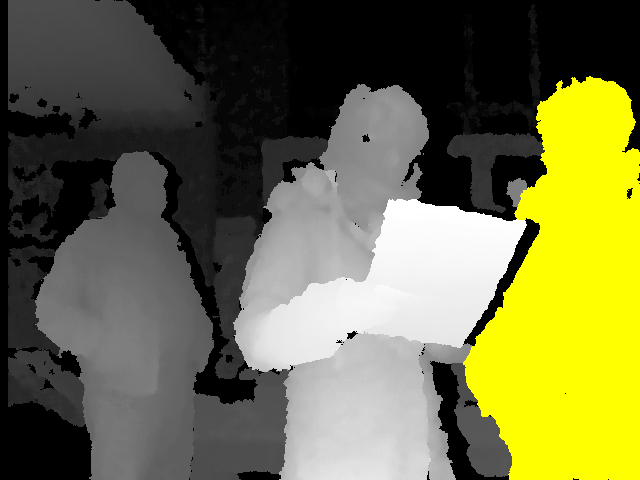
\includegraphics[width=\textwidth]{Figures/8/non_inter_findings/effects/neglegance}
        \caption{}
        \label{fig:non-blindness}
    \end{subfigure}
    \hfill
    \begin{subfigure}[H]{0.3\textwidth}
        \centering
        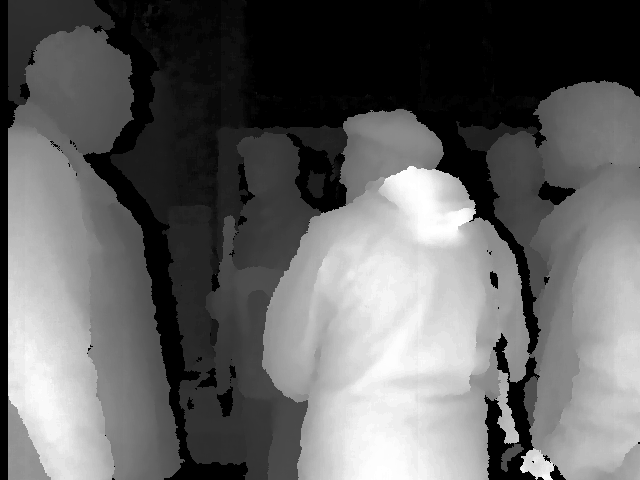
\includegraphics[width=\textwidth]{Figures/8/non_inter_findings/effects/displayblindness}
        \caption{}
        \label{fig:non-negligence}
    \end{subfigure}
    \hfill
    \begin{subfigure}[H]{0.3\textwidth}
        \centering
        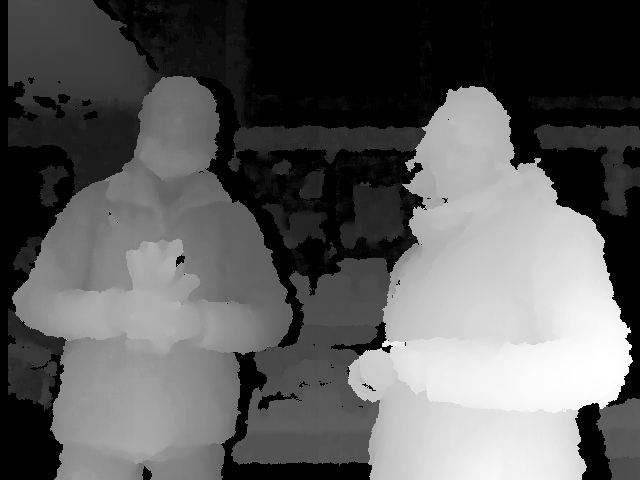
\includegraphics[width=\textwidth]{Figures/8/non_inter_findings/effects/reading}
        \caption{}
        \label{fig:non-reading}
    \end{subfigure}
    \caption{The first two pictures show that the display is completely ignored and people are busy with themselves. Picture C shows two couples are reading the screen.}
    \label{fig:three-non-behavior}
\end{figure}

\newpage
\subsection{Body Interactive findings}

\begin{enumerate}
\item \textbf{Attention Level measurements}

The bellow chart shows the observation number of glances and ignores of passers-by for two distinct hours of five days. As can be seen the in most days the number of glances and ignores are almost near but not still ignores percentage is higher, as can be seen in the pie-chart \%41.41 are the number of glances and around \%59 is the number of ignores. 
\begin{figure}[H]
    \centering
    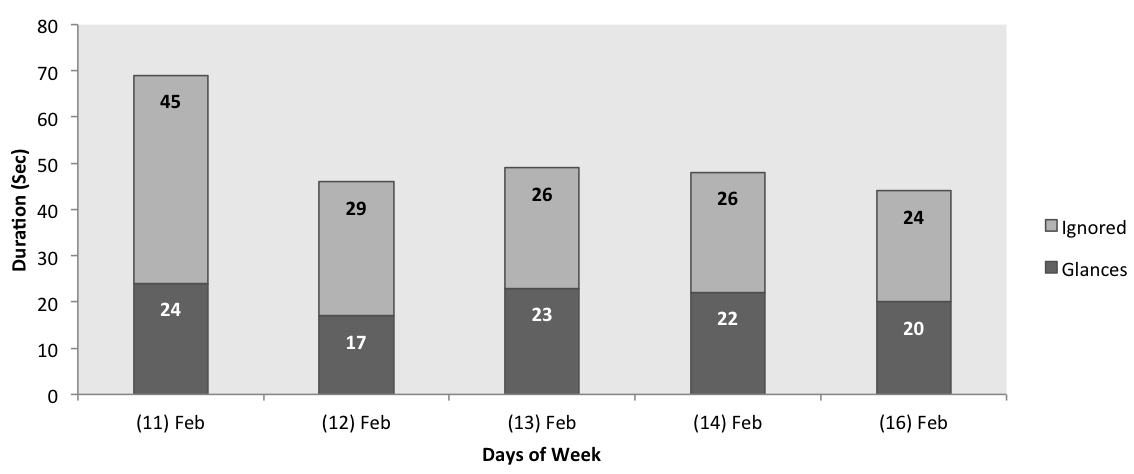
\includegraphics[width=110mm,height=60mm]{Figures/8/body_inter_findings/Body_Inter_chart}%
    \caption{Body interactive attention level chart}%
    \label{fig:bodyattentionlevelchart}%
\end{figure}


\begin{figure}[H]
    \centering
    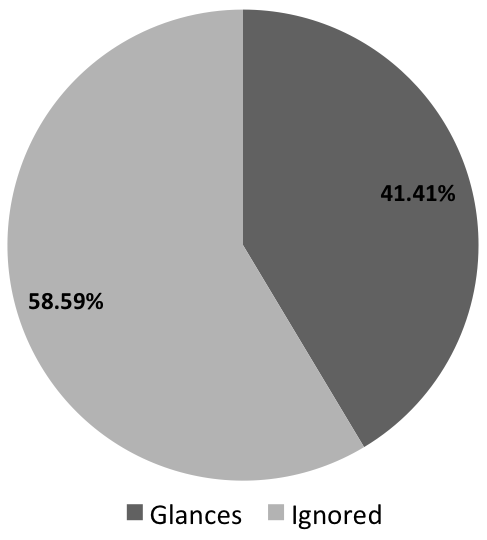
\includegraphics[width=110mm,height=60mm]{Figures/8/body_inter_findings/body_inter_percentage}
    \caption{Body interactive Attention level percentage}%
    \label{fig:bodyattentionlevelpercentage}%
\end{figure}



\item \textbf{Engagement phases and duration spent}

There were passers-by who were very interested in the interaction that played the game even three times, some people triggered the game and left in the middle and some people were just staring at the screen and did not triggered the game therefor people were engaged in different stages of the game differently and took between (10, 200) seconds and in average it took around 42 seconds.

\begin{figure}[H]
    \centering
    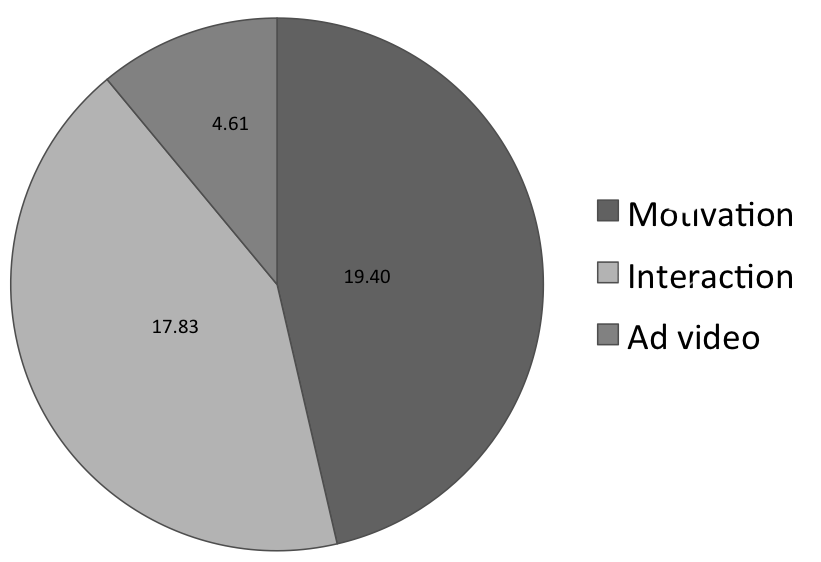
\includegraphics[width=110mm,height=60mm]{Figures/8/body_inter_findings/body_avg_phases}
    \caption{Average time for each phase}%
    \label{fig:bodyaveragephases}%
\end{figure}

The advertisement was divided in three main section (1) motivation, which is the pre-interaction phase that the participant has not started the game and just playing with body or looking to the screen or reading call-to-action text, this part was different for people some people by just looking to the screen approached and started the interaction less than 5 seconds and some people took longer time to think and then triggered the game, at some occasions participants just left without triggering the game so in average it took around 20 seconds for this stage. (2) The interaction part in which people again took different times some people played more than two or three times and some played the first element and left so in average it took about 18 seconds for this stage. (3) The advertisement video which had the least time spent most of the participants left the screen after they saw the advertisement video in 2 seconds and some were excited to play again so they waited for a while In front of display until the end of advertisement video this was very rare among participants, so in average it took around 4.5 seconds for advertisement video.


\item \textbf{Passerby and engagements} \\
We were interested that how much people pass from display and how much of them would be engaged with the display, From depth recording entire passers-by were counted along with the passers-by who got engaged with the screen the counting was done manually with the help of many computer science students.If the person who stood longer than 3 seconds was flagged as engaged.

\begin{figure}[H]
    \centering
    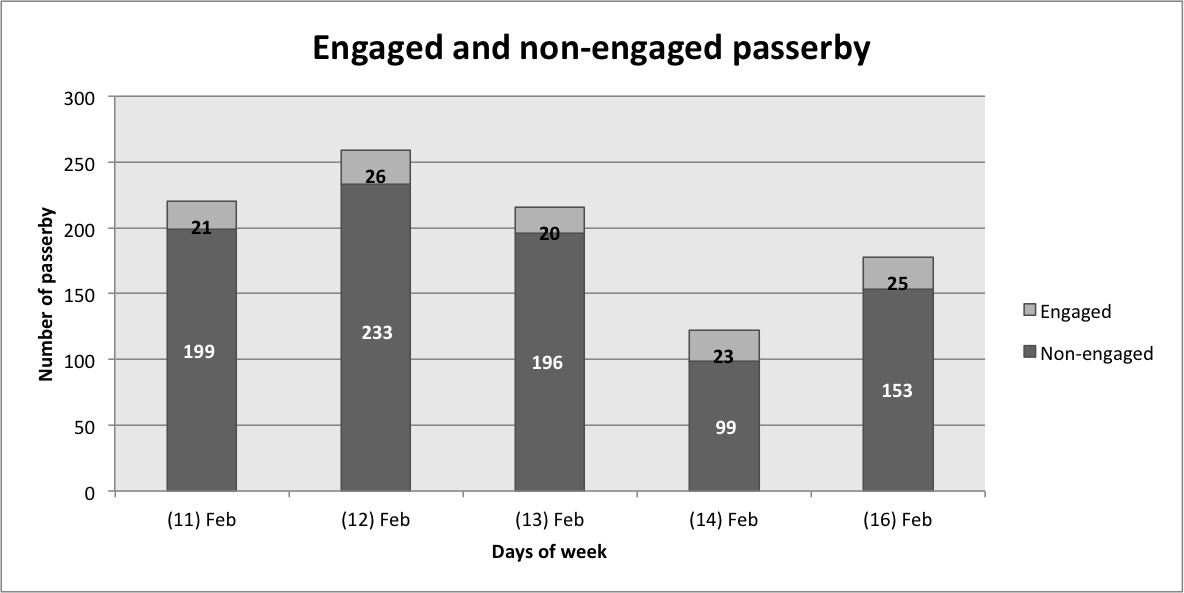
\includegraphics[width=110mm,height=60mm]{Figures/8/body_inter_findings/body_inter_engage_day}
    \caption{Body interactive Number of engaged passerby}%
    \label{fig:bodyengagedandengagedby}%
\end{figure}
As can be seen from the chart bellow the number of them are shown in bar chart for each of the day. And in average around \%12 of the passers-by were engaged with the screen. 

\begin{figure}[H]
    \centering
    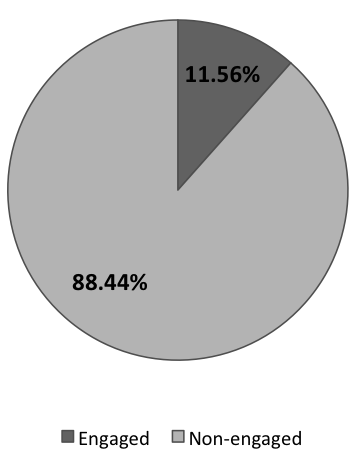
\includegraphics[width=110mm,height=60mm]{Figures/8/body_inter_findings/body_eng_percentage}
    \caption{body interactive percentage of engaged passerby}%
    \label{fig:bodyengagedpasserbypercentage}%
\end{figure}


\end{enumerate}


\newpage
\begin{enumerate}
\setcounter{enumi}{3}
\item \textbf{Landing and Honeypot effects}
\end{enumerate}

\begin{wrapfigure}{r}{0.4\textwidth}
  \vspace{-60pt}
  \begin{center}
    \includegraphics[width=0.30\textwidth,height=90mm]{figures/8/body_inter_findings/effects/landing}
  \end{center}
  \vspace{-20pt}
  \caption{Landing effect}
  \vspace{-10pt}
\end{wrapfigure}
Many landing effects and honeypot effects were observed for body interaction technique. \\
As before landing was discussed that a person recognizes the interactivity after he /she has already passed the screen, in the picture in the right the two person silhouette are projected on the screen when they are passing the second person who has yellow color (A) notices the interactivity while his friend is still continuing to pass (B, C) but the guy the person is standing to see what is going on (D) and at this point his friend notices and walks back to see the screen (E).  \\

\begin{wrapfigure}{l}{0.4\textwidth}
  \vspace{-20pt}
  \begin{center}
    \includegraphics[width=0.30\textwidth,height=90mm]{figures/8/body_inter_findings/effects/honeypot}
  \end{center}
  \vspace{-20pt}
  \caption{Honeypot Effect}
  \vspace{-20pt}
\end{wrapfigure}

The honeypot effect is the effect that other people are attracted by noticing the current people that are somehow involved (interacting) with the display.

The picture on the left shows a boy interacting with the system (A) when the body move a bit behind from the display (B) at this time another random person who does not know him notices him or has notice before, tries to approach to the screen (C) and then when the person sees himself then from he actively tries to take control of the interaction (D) and the other active person was left behind the scene.

The bellow chart lists all the frequencies of honeypot effect and landing effects that was recorded from the depth recordings and onsite observations.   \\ \\


\begin{table}[H]
\caption{Body Interactive Landing and honeypot effect}
\label{tab:landingandhonypot_body}
\centering
\begin{tabular}{| l | c | c |}
\toprule
\tabhead{Days} & \tabhead{Landing effect} & \tabhead{Honeypot effect} \\
\midrule
\textbf{11 Feb}  & 2 &  2 \\
\textbf{12 Feb}  & 3 &  3 \\
\textbf{13 Feb}  & 2 &  2 \\
\textbf{14 Feb}  & 2 &  5 \\
\textbf{16 Feb}  & 3 &  3 \\
\bottomrule
\end{tabular}
\end{table}

\newpage


\begin{enumerate}
\setcounter{enumi}{4}
\item \textbf{Interviews} \\
The interviews were coded each individually and as a result the bellow categories are extracted, these categories are mainly taken from the questions and others are from the replies of the participants. 

\begin{enumerate}

\item Noticing \\
    Different people had their different experience and reaction when they noticed themselves in the display for the first time. Some of the people were standing and looking some books for long time when they saw themselves and for confirmation they waved toward the screen, as one said ``\emph{Yes at first I thought that it is not me. I waved my hand and came near.}'' Other said, ``\emph{Yes I saw my blue color body}''. Other participants noticed at the time of passing from front of the screen, ``\emph{when I was passing I saw myself in the screen.}'' Other people saw their friend first then noticed themselves like one said, ``\emph{I saw my friend in the screen and came near and I was also there with blue color.}'' One participant who usually comes to the center every week said that because the screen was newly installed I came near to the screen to see what is new inside.

\item Ad recall \\
    Respondents responded accurately the content and goal of the advertisement as one said, ``\emph{It was about a tour of Bauhaus, Bauhaus Spaziergang.}'' ``\emph{It was about tour in the city.}'' And other said, ``\emph{It was about Bauhaus-Walk. City tour.}'' And other said, ``\emph{it is something to do with Bauhaus city walk}''.

\item Interest \\
    People find this type of interaction very interesting, funny and motivative, one participant mentioned that, ``\emph{I liked to see myself in the screen, it was funny.}'' Other says the use of media is very interesting and comfortable for people, ``\emph{I think that the people with the use of media is comfortable}''. The use of this type of interactive advertisement give people some sort of good feeling toward Bauhaus-Walk event like one said, ``\emph{Bauhaus is very interested to me and it sounds fun}''. People also liked the way content was inside the advertisement like one said, ``\emph{It is very interesting to see the pictures}'' and even one participant exactly mentioned the goal of the advertisement interaction, ``\emph{it was a very interesting idea and it is like a small interactive tour for the people who want to take Bauhaus-Walk.}''

\item Event participation  \\
    Respondents showed sign of interest to join the program in future but are not able to join quickly because of many reasons like they are here for short visit as one said, ``\emph{We are here in Weimar for short visit}'', others said they are busy with many other programs like one said, ``\emph{Now we are going to Weimar Museum}''.

\item Confusions \\
    There was some confusion during interaction, like the interaction seemed unclear, one said, ``\emph{I did not understand how it works}'' other said, ``\emph{I left because I did not understand}'' and some people also experienced this by coming very close to the screen and nothing is shown to them at that time, ``\emph{when I was standing I saw that it says come near, and I came near to the screen and the map came but I left after standing for a short time because I did not understand it.}''

\item Dislikes \\
    When a person hovers on a location in the map, a related picture is shown on the screen and deems off after a while, some participants complained about time and said, ``\emph{Pictures goes very fast}'', one person complained about the rendering speed and said, ``\emph{Pictures come very late}''.

\item Recommendations  \\
    Respondents recommended that the advertisement should be able to hint users on how to use it, as one said, ``\emph{It would be good to put some more information that how we can use it.}''  Other said that ``\emph{Maybe explain how someone can walk with these body figures}''. One person even said, ``\emph{It is good that here someone stand and describe it to the people who come near to the screen.}'' Some of the participants also recommended to slow down the picture changing of the advertisement.

\end{enumerate}



\newpage

\item \textbf{Other observations} \\
\emph{fix the note taking}
check appendix \ref{AppendixD}.9 and \ref{AppendixD}.10


During the body interactions despite honeypot and landing effect other different kinds of behaviors have been observed and how passers-by reacted when there was an interactive display, the behavior with the display was much different compared to non-interactive as listed bellow.

\begin{itemize}
\item Group interaction \\
Most of the passers-by interacted when they were in a group maybe they felt much secure and confident, and mostly their interaction last longer, few individual participants interacted with the display which was shorter compared to group interaction. The bellwo pictures show group interaction between two friends In (A, B) and another three persons in (C, D). 

\begin{figure}[H]
    \centering
    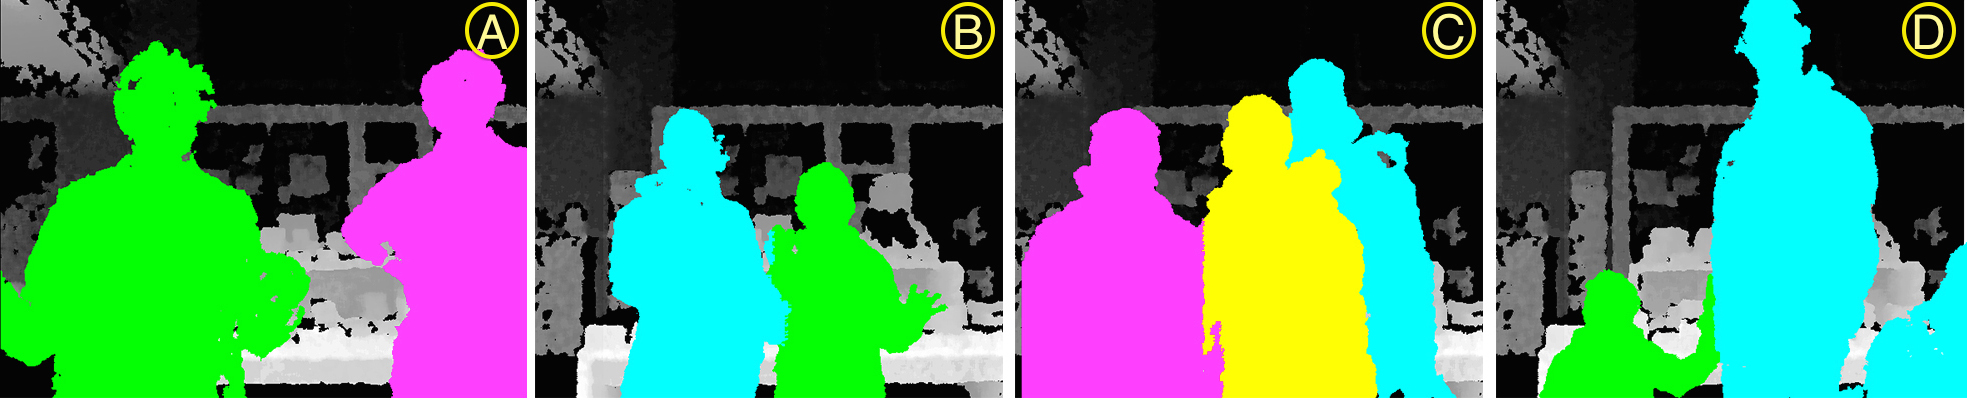
\includegraphics[width=100mm,height=30mm]{Figures/8/body_inter_findings/effects/group}
    \caption{}
    \label{fig:group_interaction}
\end{figure}


\item Calling others
People were getting really excited and liked to call his / her friends to come and join and have fun with the interaction, most of this reaction was seen between children and parents and couples. As can be seen in frame (A) a person is watching the display and then moves out in frame (B) and in frame (C) calls a friend of him/her and in frame (D) both of them are in center of the screen and watching themselves in it.


\begin{figure}[H]
    \centering
    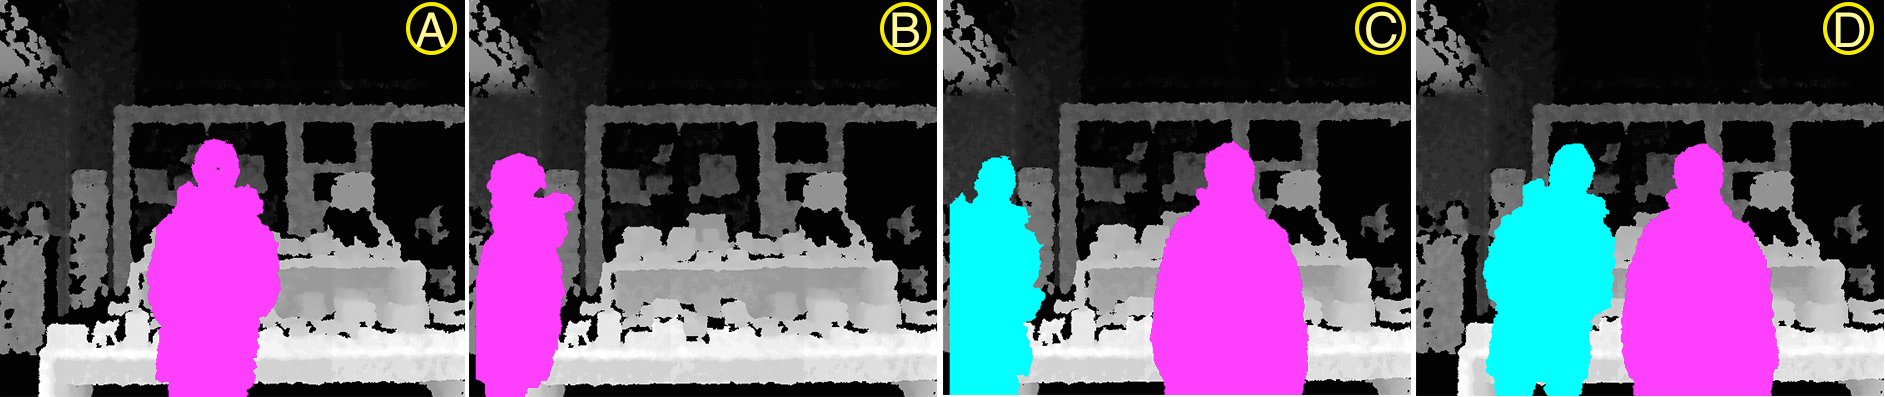
\includegraphics[width=100mm,height=30mm]{Figures/8/body_inter_findings/effects/calling_others}
    \caption{Calling others}
    \label{fig:calling_interaction}
\end{figure}


\item Playing with silhouette  \\
Passers-by liked the different colors specially when they were couples or children before they triggered the interaction. As can be seen in bellow picture there is a couple that likes to play with the different colors of their silhouette.

\begin{figure}[H]
    \centering
    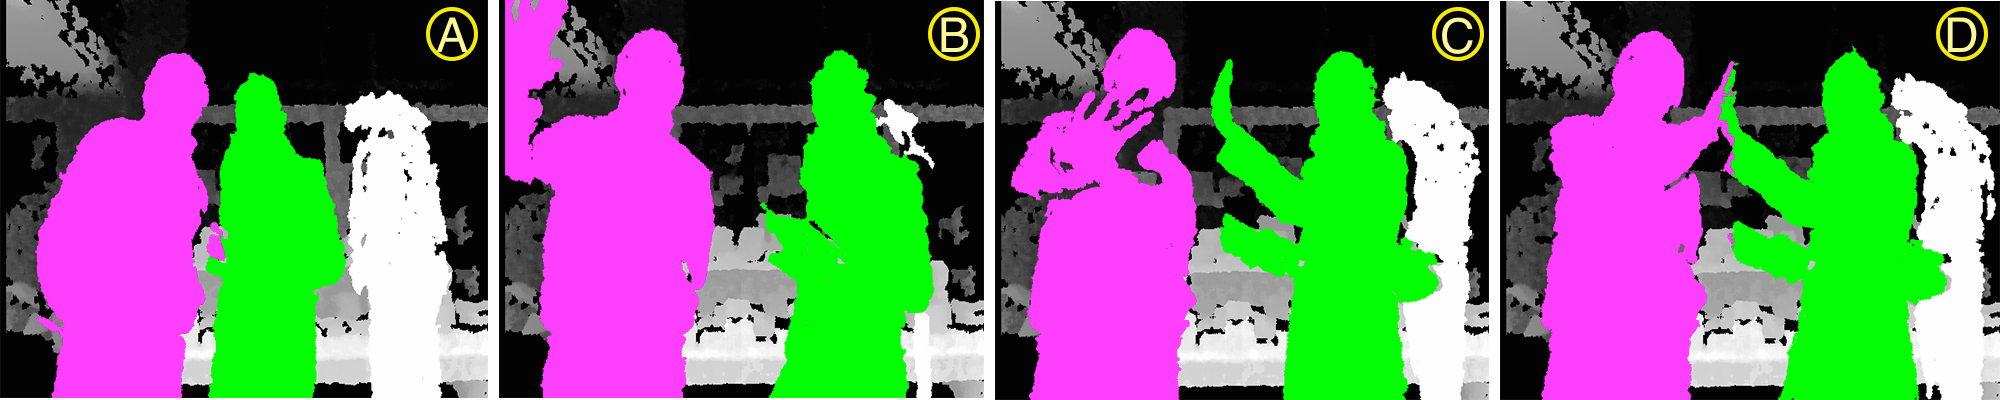
\includegraphics[width=100mm,height=25mm]{Figures/8/body_inter_findings/effects/playing}
    \caption{Playing with silhouette}
    \label{fig:playing_interaction}
\end{figure}


\item Interactivity confirmation \\
People who saw their selves from far distance were not sure if the screen was interacted so they started waving their hands, body or their heads to see if their silhouette reacts to their movements. Some of the people did not apparently acted but progressively came near to screen like (spying) and then left. As can be seen in bellow frames, in (A) a person notices his/her silhouette and immediately raises hands in frame (B) and his fellow friend also notices and raises hand up in (C and D).

\begin{figure}[H]
    \centering
    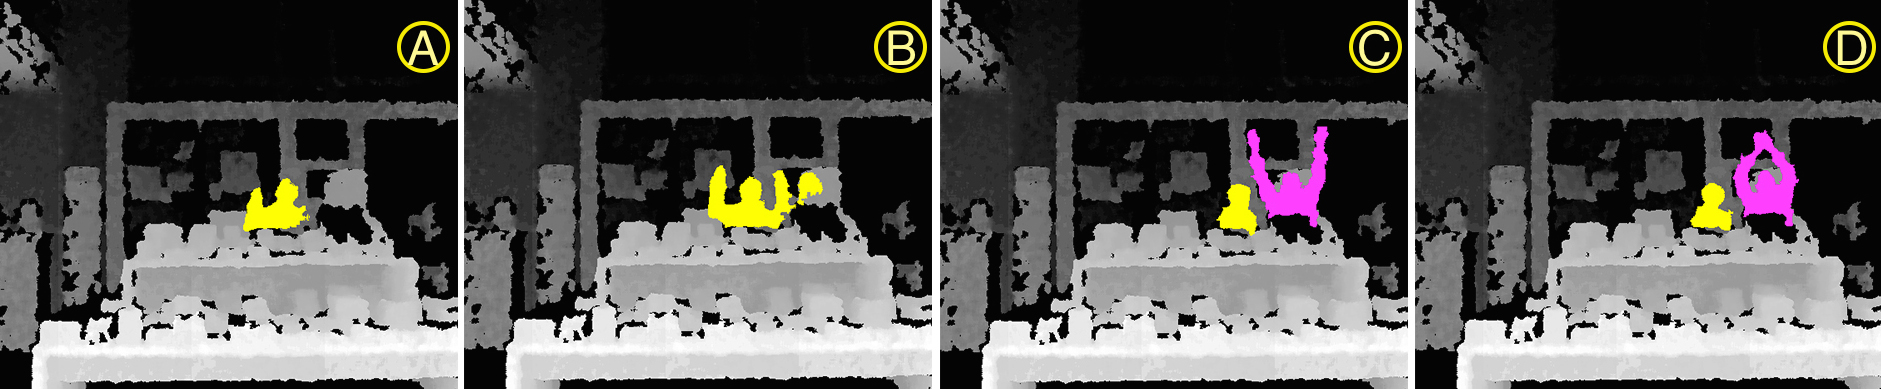
\includegraphics[width=100mm,height=30mm]{Figures/8/body_inter_findings/effects/noticing}
    \caption{Noticing interactivity}
    \label{fig:noticing_interactivity}
\end{figure}
 

\item Raising hands up \\
During the interactions some of participants raised their hands up mainly because of the alert message that was shown on top right corner of the screen if they were undetected by Kinect camera. As can be seen in the pictures that shows different frames people during interaction and prior to interaction are raising their hands up. 

\begin{figure}[H]
    \centering
    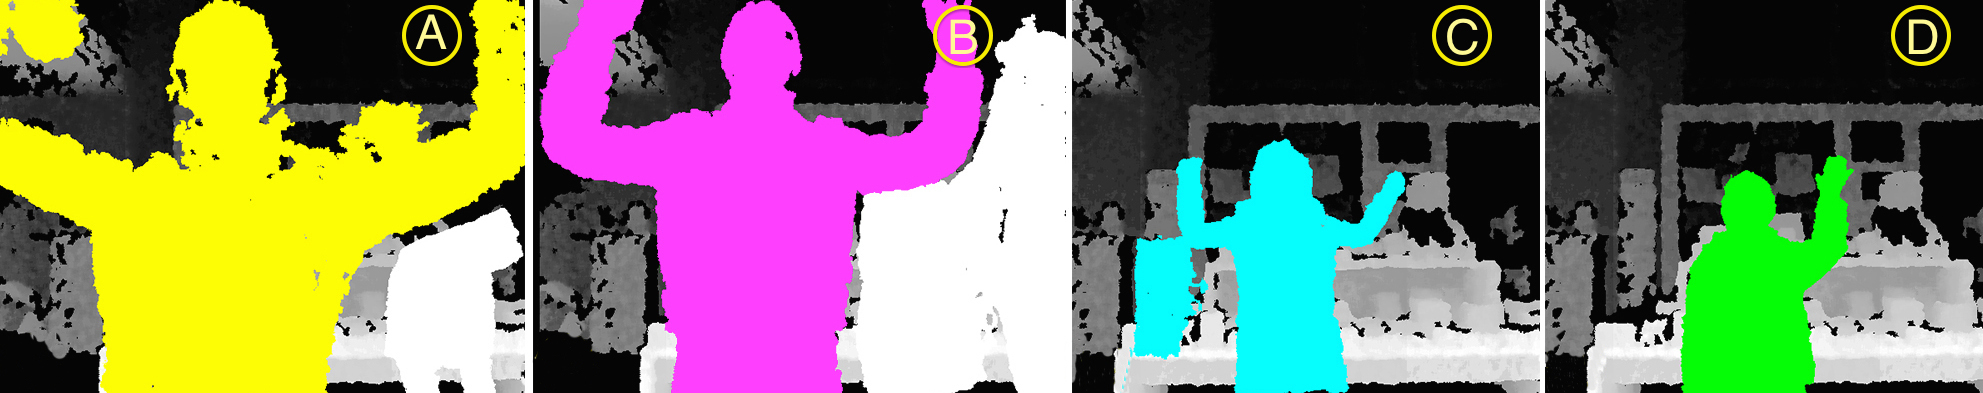
\includegraphics[width=100mm,height=30mm]{Figures/8/body_inter_findings/effects/raisinghand}
    \caption{Raising hand}
    \label{fig:raisinghand_interactivity}
\end{figure}


\item Physical space domination \\
The people in front of the display were either interacting or either leaving the space by walking away or turning their face back from display, people felt some sort of influence of their presence in front of it. 

\item Call-to-action reaction \\
Most people came very close to the screen when approached by the application, this lead to confusion later in interaction because the camera could not longer track them.

\item Interactions behaviors \\
The movement of silhouette during interaction is by moving forward / backward or left / right, some at early interaction leaned down or jumped higher to go forward or backward on the map.


\item Incorrect expectations \\
Some passers-by who started the interaction using their body, expected that the screen should be working using touch, they tried many times to touch the elements, one of the main reason of this behavior seemed to relied on the fact that they were called to come near, and they felt became more personal with the display and the display which was small in dimension also provides the hint of being personal. Touch interaction is know to be more personal action than using body or other gestures. 


\item Interaction negligence (technology skeptical) \\
Some of the elder participants ignored the interaction even after understanding the call-to-action, and after interviewing them they responded that they did not know how that thing works, and after interviewing an employee of the tourist information, he said that the elders are a bit skeptical about the use of technology. 

\end{itemize}




\newpage
\subsection{Mobile Interactive findings}


\item Attention Level measurements
Attention attraction technique was quite similar to body interaction technique, which was projection passers-by silhouette but with a difference of access information text rendered on top, people would partially see their silhouette but still it was an attention mechanism, the measurement was done for five days each day for only two hours of direct observation. 


\begin{figure}[H]
    \centering
    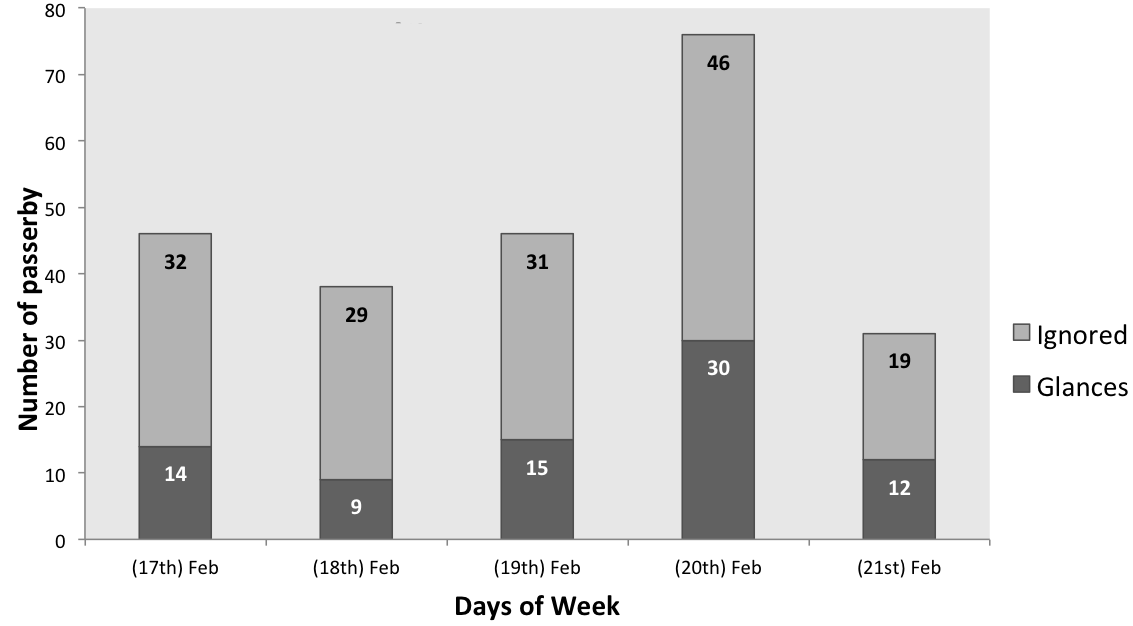
\includegraphics[width=110mm,height=60mm]{Figures/8/mobile_inter_findings/mobile_Inter_chart}%
    \caption{Mobile interactive attention level chart}%
    \label{fig:mobileattentionlevelchart}%
\end{figure}

As can be seen the number of glances have decreased compared to body interaction, since other things were not changed except for the access information so it could be the result of that, that people have not fully seen themselves or recognized. 

\begin{figure}[H]
    \centering
    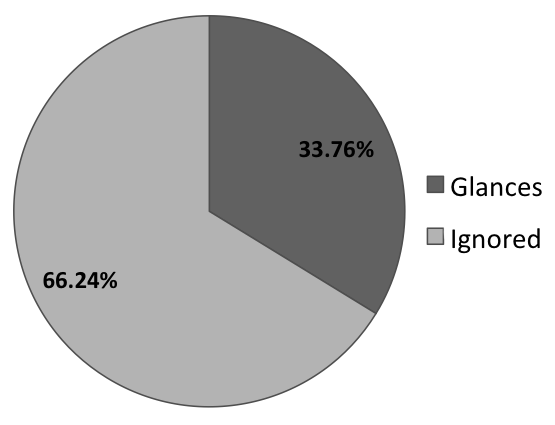
\includegraphics[width=110mm,height=60mm]{Figures/8/mobile_inter_findings/mobile_inter_percentage}
    \caption{Mobile interactive Attention level percentage}%
    \label{fig:bodyattentionlevelpercentage}%
\end{figure}
The percentage of the whole week of glances was around \%34 and \%66 of the cases the screen was ignored.

\item \textbf{Engagement time}

Although no passers-by interacted with the system, all of the participants were in the first screen of the advertisement that showed the Bauhaus-walk name and their silhouette. It took in average around 22 seconds to be engaged passively with the screen, which is less than non-interactive and body interactive applications. 


\item \textbf{Passerby and engagements}
The entire five days were observed using the depth recordings and manually the number of passers-by were counted and from which the passers-by who stood for more than 3 seconds were flagged as engaged, as can be seen bellow in pie chart that shows one day each. Most of the passers-by stood for a very short time. 

\begin{figure}[H]
    \centering
    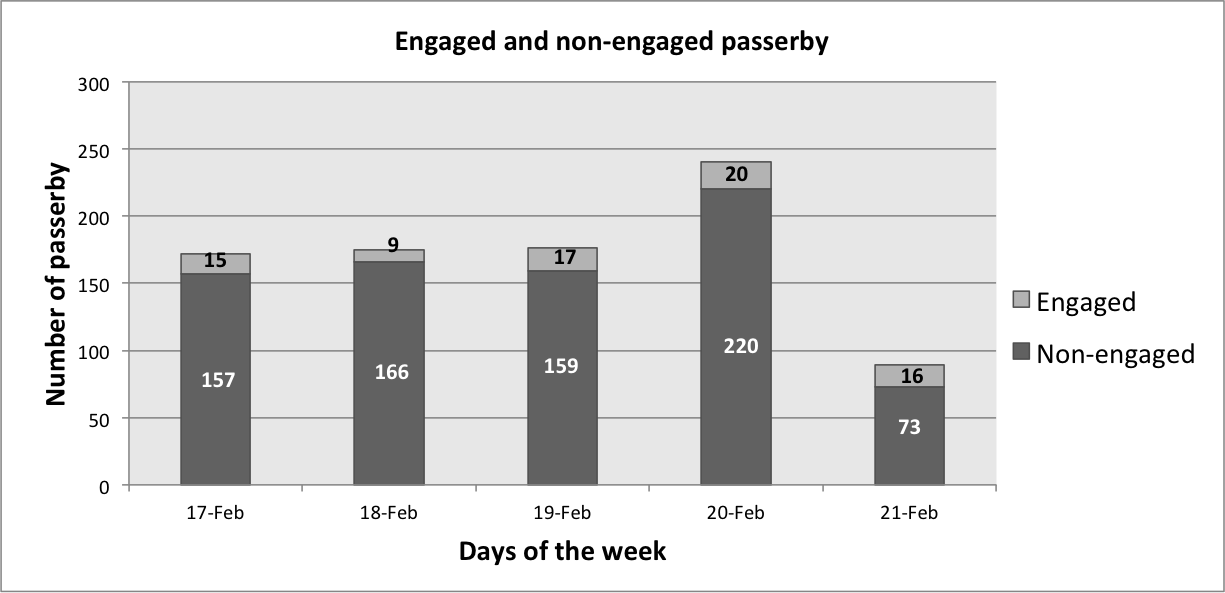
\includegraphics[width=110mm,height=60mm]{Figures/8/mobile_inter_findings/mobile_inter_engage_day}
    \caption{Mobile interactive Number of engaged passerby}%
    \label{fig:mobileengagedandengagedby}%
\end{figure}

Only \%9 of the passers-by were engaged with the system.


\begin{figure}[H]
    \centering
    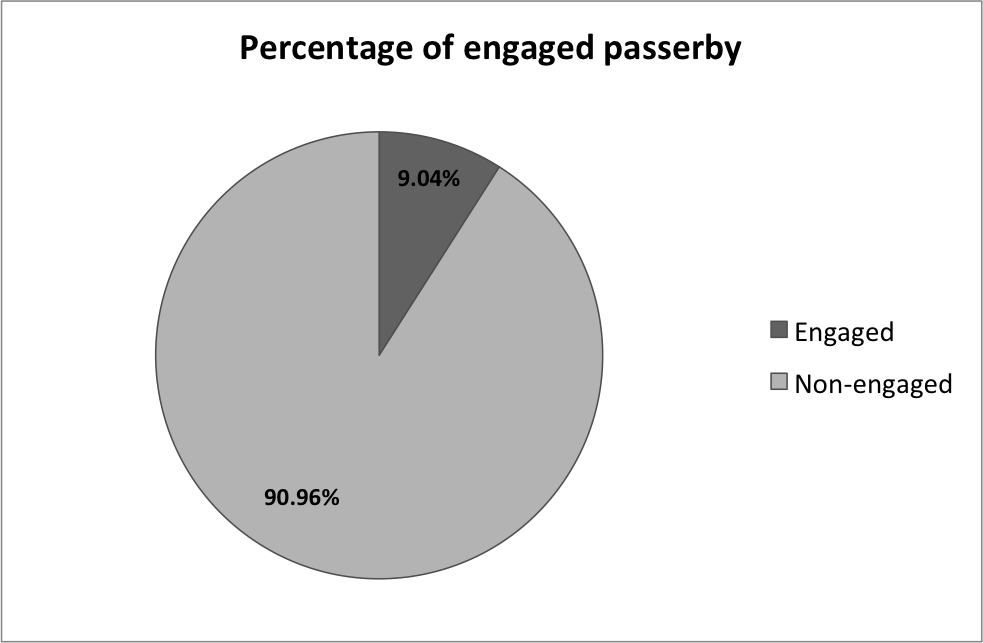
\includegraphics[width=110mm,height=60mm]{Figures/8/mobile_inter_findings/mobile_eng_percentage}
    \caption{Mobile interactive percentage of engaged passerby}%
    \label{fig:mobileengagedpasserbypercentage}%
\end{figure}



\end{enumerate}

\newpage

\begin{enumerate}
\setcounter{enumi}{3}

\item \textbf{Landing and Honeypot effects}
\end{enumerate}

Landing and honeypot effects in this technique were very not strong enough mainly because no passers-by interacted with the system.

Honeypot effect was mainly because of the silhouette representation as said before this effect was very week because of info-screen that showed partial body representation, passers-by rarely noticed the text. Only two times honeypot effect occurred and people did not get engaged with the system afterward. This effect could have been improved if passers-by had actively participated to play game.  The picture bellow shows a green colored person at frame (A) at this point he was watching the screen for a while and when he moves out of the screen (B, C) another yellow colored person appears from the back side (C) and walks toward the screen (D, E) and gets close very close (F).

\begin{figure}[H]
    \centering
    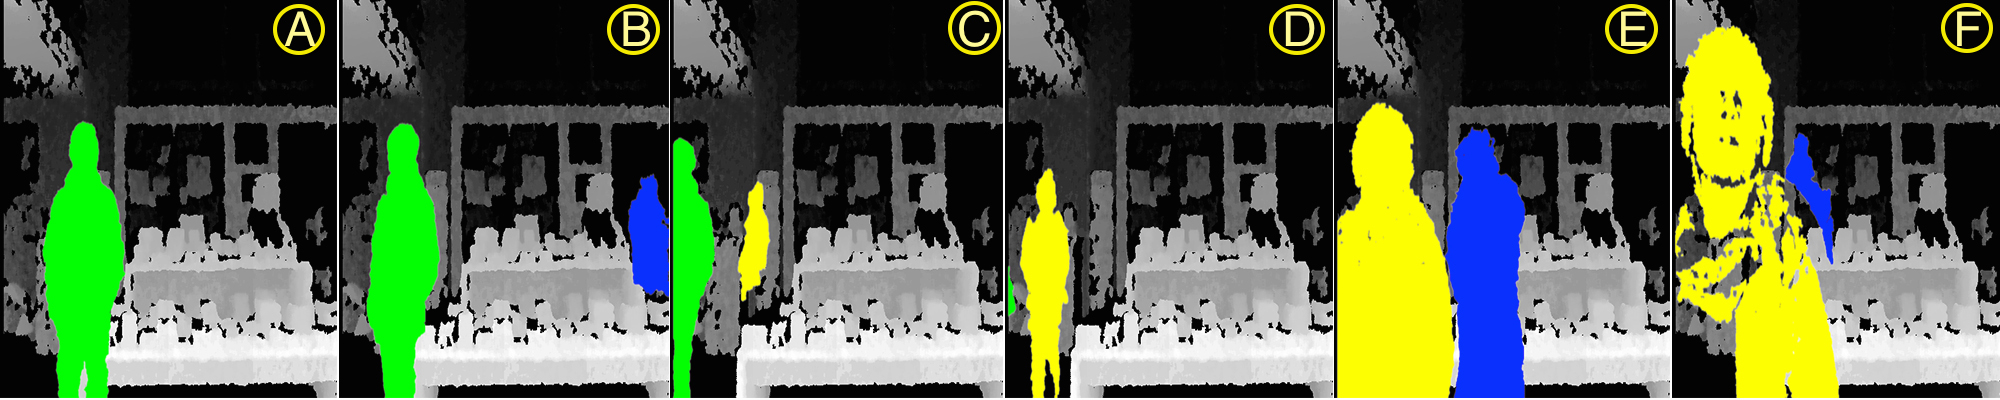
\includegraphics[width=100mm,height=25mm]{Figures/8/mobile_inter_findings/effects/honeypot}
    \caption{Honeypot effect}
    \label{fig:mobile_honeypoteffect}
\end{figure}


Landing effect was also recorded in some occasions and mainly happened because they saw their silhouette, very less people noticed and most ignored as shown in the picture from right to left a person is crossing the screen (A – E) but on frame (F) stops and move a little back to see what is on the screen. The person does not entirely come in the center of the screen.

\begin{figure}[H]
    \centering
    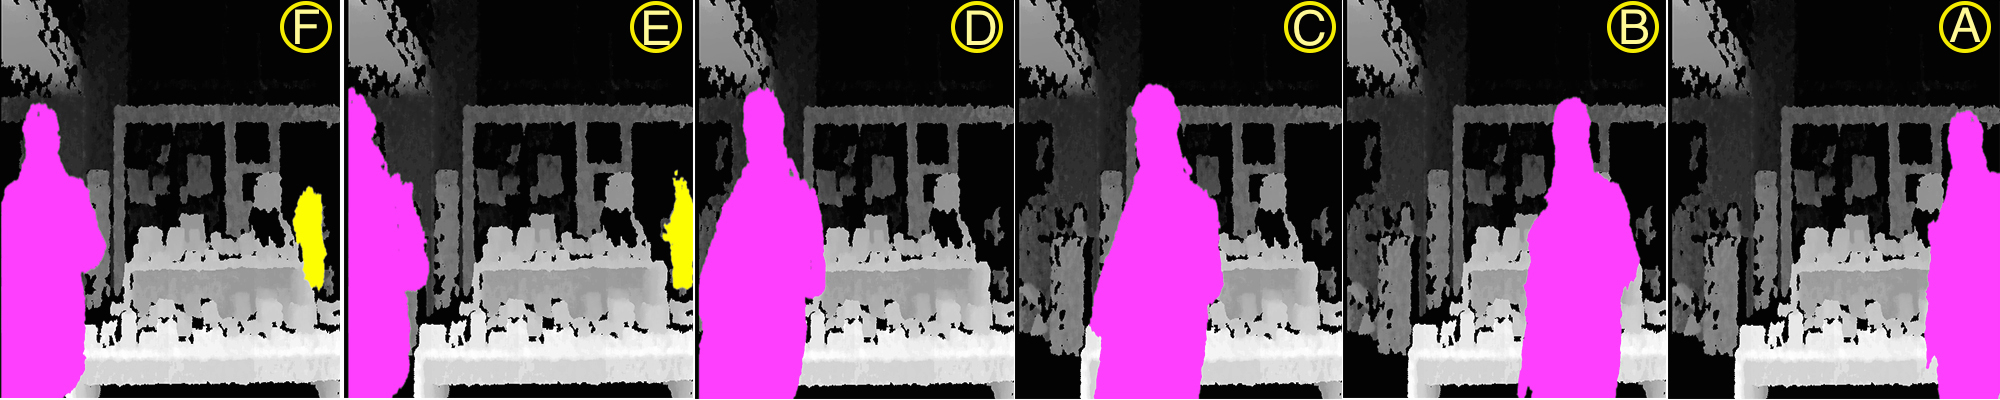
\includegraphics[width=100mm,height=25mm]{Figures/8/mobile_inter_findings/effects/landing}
    \caption{Landing effect}
    \label{fig:mobile_landingeffect}
\end{figure}




\begin{table}[H]
\caption{Mobile Interactive Landing and honeypot effect}
\label{tab:landingandhonypot_mobile}
\centering
\resizebox{8cm}{1.5cm}{
\begin{tabular}{| l | c | c |}
\toprule
\tabhead{Days} & \tabhead{Landing effect} & \tabhead{Honeypot effect} \\
\midrule
\textbf{17 Feb}  & 0 &  1 \\
\textbf{18 Feb}  & 1 &  0 \\
\textbf{19 Feb}  & 2 &  0 \\
\textbf{20 Feb}  & 0 &  0 \\
\textbf{21 Feb}  & 1 &  1 \\
\bottomrule
\end{tabular}
}
\end{table}



\begin{enumerate}
\setcounter{enumi}{4}

\item \textbf{Interviews}


\hilight{complete the interview report}


\newpage
\item \textbf{Other observations}

\hilight{fix Appendix \ref{AppendixD}.11}

Passers-by were attracted to the system when they saw their silhouette, which was kind of similar to the body interaction technique. The bellow are behaviors people had with the system.

\begin{itemize}
\item Curiosity \\
Passers-by who noticed showed curiosity and tried to come near to the screen or started waving their hands toward the screen.
 
\item Interaction ignoring \\
All the people who were attracted ignored to interact, that could have many different reasons, like the lack of enough knowledge of how to do, or not having mobile phones or not interested to play, as one of them were interviewed he said that he does not use phone for in public he only uses it for calling. 

\item Scanning code \\ 
During five days only two persons tried to scan the QR-code and after scanning they just left.

\item Playful   \\
Most of the kids that noticed felt excited only to see their different colored silhouette and even at some point started to dance in group. 



\item Inappropriate physical space \\
Because most of the passers-by pass and do not expect interaction with the displays and especially with mobile phone would be very difficult to be convinced because the screen is situated in the pathway of people, people would not interact with phone standing. I believe for mobile interaction it would be nice to place display where people can sit and interact.

\item Limited time \\
Passers-by have limited time to pass the screen and by mean time they should be convinced to start interaction, but as found out in the usability testing of mobile phone in previous chapter, it take much longer to understand how to start the game, this results to ignore the interaction with the smartphone. 

\item Being skeptical \\
The old generation are most of them skeptical about using technology and specially things that are their own like mobile phones, even though having a smartphone they do not tend to use their phone for public use and in this case for an advertisement. 

\item Feeling unsecure \\
Some people may thing unsecure of using their personal phone, thinking that maybe other information may be extracted from their phones, so they try to stay away from using their phones in public space. 


\end{itemize}




\end{enumerate}


\newpage
\subsection{Comparison of advertisements}

\subsubsection {Number of passerby}
Because the advertisements techniques were not conducted in the same days, which could ruin comparison because of different number of passers-by everyday and each week, there was a need to first compare the number of passers-by and prove that they were not statistically different in between. \\

\textbf{Hypothesis: }
\begin{itemize}
\item \textbf{H0:} There was no difference between numbers of passerby of each week.
\item \textbf{H1:} There was a difference between numbers of passerby of each week.
\end{itemize}

The bellow is the table of passerby for three weeks.

\begin{table}[H]
\caption{Number of passerby in three weeks}
\label{tab:passerbyofthreeweeks}
\centering
\resizebox{8cm}{1.5cm}{
\begin{tabular}{| l | c | c | c |}
\toprule
\tabhead{Days} & \tabhead{First week} & \tabhead{Second week} & \tabhead{Third week} \\
\midrule
\textbf{Day 1}  & 232 & 178 &  172 \\
\midrule
\textbf{Day 2}  & 170 & 220 &  175 \\
\midrule
\textbf{Day 3}  & 212 & 259 &  176 \\
\midrule
\textbf{Day 4}  & 209 & 216 &  240 \\
\midrule
\textbf{Day 5}  & 208 & 122 &  89  \\
\midrule
\textbf{Total}  & 1031 & 995 & 852 \\
\bottomrule
\end{tabular}
}
\end{table}

ANOVA test revealed that there is no significant different of passers-by between each of the weeks.
 \emph{(F2,5)=0.8873, p >.05 (p=0.437)}
 So based on this the \emph{H0} hypothesis is being accepted and \emph{H1} hypothesis is being rejected. This gives us confidence to proceed our comparisons.



\subsubsection {Attention Level Comparison}

As can be seen Non-interactive (first week) had \%28.83 number of glances, the Body-interaction (second week) had almost \%10 high number of glances (\%38.70) than non-interactive, The mobile Interaction had higher glances (\%33.75) from non-interactive but still less than body interaction. But with this we can not conclude that body interaction had higher until we statistically state them.

To compare which of the the three methods drove more passers-by attention, the data of number of glances for each of the weeks are gathered as bellow and first we want to find out if these data are statistically different or not.\\

\textbf{Hypothesis: }
\begin{itemize}
\item \textbf{H0:} There was no difference between numbers of passerby of each week.
\item \textbf{H1:} There was a difference between numbers of passerby of each week.
\end{itemize}



% table
\begin{table}[H]
\caption{Cross tabulation for each week attention level }
\label{tab:crosstabulationweeks}
\centering
\resizebox{8cm}{1.5cm}{
\begin{tabular}{| l | c | c | c |}
\toprule
\tabhead{Method} & \tabhead{Glanced (\%)} & \tabhead{Ignored} & \tabhead{Total } \\
\midrule
\textbf{First week}     & 111(\%28.83)   &   274      &   385\\
\midrule
\textbf{Second week }   & 106 (\%41.41)   &   150      &   256\\
\midrule
\textbf{Third week }    & 80 (\%33.75)   &   157      &   237\\
\midrule
\textbf{Total }         & 297            &   581      &   878\\
\bottomrule
\end{tabular}
}
\end{table}



Running Chi-squared test to see the significant between different advertisement conditions and the bellow result shows that they are statistically significant.
${\chi}^2$\emph{(2, N=878)=10.863, p < .05 (p=.004376)}, so \emph{H0} is rejected and \emph{H1} hypothesis would be accepted.
To find the actual difference, each pairs were tested in between using again Chi-squared test.

\begin{enumerate}
\item Non-Interactive Vs Body Interactive \\
The finding shows that body interactive advertisement had significant number of glances than non-interactive advertisement. \\
${\chi}^2$\emph{(1, N=641)=10.8581, p < .005 (p=.000984)}

\item Non-Interactive Vs Mobile Interactive  \\
The finding suggests that there is no significant difference between Non-interactive and mobile in this case.\\
${\chi}^2$\emph{(1, N=622)=1.6716, p > .05 (p=.196039)}

\item Body interactive Vs Mobile Interactive \\
As can be expected the glances are not statistically significant among the body and mobile interactive advertisement too.\\
${\chi}^2$\emph{(1, N=493)=3.0663 , p > .05 (p=.07993)}

\end{enumerate}


\subsubsection {Engaged and Non-engaged passers-by}
This test is to find out if there is a difference between number of Engaged passerby or not between the weeks.

\textbf{Hypothesis: }
\begin{itemize}
\item \textbf{H0:} There is no difference between the numbers of Engaged passerby between the weeks.
\item \textbf{H1:} There is a difference between the numbers of Engaged passerby between in each weeks.
\end{itemize}

The bellow table lists all number of engaged and non-engaged passers-by for three weeks.


\begin{table}[H]
\caption{Number of engaged passers-by in three weeks}
\label{tab:engagedofthreeweeks}
\centering
\resizebox{8cm}{1.5cm}{  
\begin{tabular}{| l | c | c | c |}
\toprule
\tabhead{Days} & \tabhead{First week} & \tabhead{Second week} & \tabhead{Third week} \\
\midrule
\textbf{Day 1}  & 16 & 25 &  15 \\
\midrule
\textbf{Day 2}  & 18 & 21 &  9 \\
\midrule
\textbf{Day 3}  & 15 & 26 &  17 \\
\midrule
\textbf{Day 4}  & 15 & 20 &  20 \\
\midrule
\textbf{Day 5}  & 15 & 23 &  16  \\
\midrule
\textbf{Total}  & 79 & 115 & 77 \\
\bottomrule
\end{tabular}
}
\end{table}

The ANOVA test strongly suggests that there is a significant difference of the number of Engaged passersby between these three weeks.\\
 \emph{(F2,5)=11.20, p >.05 (p=.002)}

To find where are the main difference between them are, the Post-Hoc Tukey’s HSD test was conducted on each three pairs of the week to point out which of them exhibit statistically significant difference. 


\begin{table}[H]
\caption{Post-Hoc Tukey’s HSD}
\label{tab:engage-non-posthoctukey}
\centering
\resizebox{\textwidth}{!}{  
\begin{tabular}{| l | c | c | c |}
\toprule
\tabhead{Methods} & \tabhead{Tukey HSD Q statistic} & \tabhead{Tukey HSD p-value} & \tabhead{Tukey HSD inferfence} \\
\midrule
\textbf{A vs B}  & 5.6337 & 0.0047509 & \cellcolor{green!80} ** p<0.01  \\
\midrule
\textbf{A vs C}  & 0.3130 & 0.8999947 &  \cellcolor{red!80} insignificant \\
\midrule
\textbf{B vs C}  & 5.9467 & 0.0032197 & \cellcolor{green!80} ** p<0.01 \\

\bottomrule
\end{tabular}
}
\end{table}


Method A, B and C refers to (Non-interactive, body interactive and mobile interactive) advertisement accordingly. As can be seen from the above chart, there is no significant difference between group A and C and group B which is body interactive advertisement shows a significant difference between A and C. it shows that the body interactive advertisement engaged significantly more passersby than other two types of advertisement.


\subsubsection {Landing effect}
The bellow table shows how many landing effects were recorded from the depth observation video for each of the weeks.\\


\textbf{Hypothesis: }
\begin{itemize}
\item \textbf{H0:} There is no difference between the numbers of Engaged passerby between in each week.
\item \textbf{H1:} There is a difference between the numbers of Engaged passerby between in each week.
\end{itemize}

\begin{table}[H]
\caption{Number of Landing effect in three weeks}
\label{tab:landingeffectthreeweeks}
\centering
\resizebox{8cm}{1.5cm}{  
\begin{tabular}{| l | c | c | c |}
\toprule
\tabhead{Days} & \tabhead{First week} & \tabhead{Second week} & \tabhead{Third week} \\
\midrule
\textbf{Day 1}  & 1 & 2 &  0 \\
\midrule
\textbf{Day 2}  & 0 & 3 &  1 \\
\midrule
\textbf{Day 3}  & 2 & 2 &  2 \\
\midrule
\textbf{Day 4}  & 0 & 2 &  0 \\
\midrule
\textbf{Day 5}  & 1 & 3 &  1  \\
\bottomrule
\end{tabular}
}
\end{table}

ANOVA test reveals that there is a significant difference between one or two above conditions, ( \emph{(F2,5)=7.529, p >.05 (p=.008)}). So we reject the Null hypothesis and state that one of the above conditions are statistically significant from the others, to confirm this we again run Post-Hoc Tukey’s HSD test on the above data.


\begin{table}[H]
\caption{Post-Hoc Tukey’s HSD results}
\label{tab:landing-non-posthoctukey}
\centering
\resizebox{\textwidth}{!}{ 
\begin{tabular}{| l | c | c | c |}
\toprule
\tabhead{Methods} & \tabhead{Tukey HSD Q statistic} & \tabhead{Tukey HSD p-value} & \tabhead{Tukey HSD inferfence} \\
\midrule
\textbf{A vs B}  & 4.7527 & 0.0144554 & \cellcolor{green!50} * p<0.05  \\
\midrule
\textbf{A vs C}  & 0.0000 & 0.8999947 &  \cellcolor{red!80} insignificant \\
\midrule
\textbf{B vs C}  & 5.9467 & 0.0144554 & \cellcolor{green!50} * p<0.05 \\

\bottomrule
\end{tabular}
}
\end{table}


Group A, B and C refers to (Non-interactive,body interactive and mobile interactive) advertisement accordingly As can be seen the test shows that the condition A and C are insignificant but condition B is significant from A and C, which means that body interactive advertisement has statistically higher landing effects than other 


\subsubsection {Honeypot effect}
The bellow table shows how many honeypot effects were recorded from the depth observation video.\\

\textbf{Hypothesis: }
\begin{itemize}
\item \textbf{H0:} There is no significant difference between the numbers of honeypot effect for the above three advertisement types.
\item \textbf{H1:} There is significant difference between the numbers of honeypot effect for the above three advertisement types.
\end{itemize}


\begin{table}[H]
\caption{Number of Honeypot effect in three weeks}
\label{tab:landingeffectthreeweeks}
\centering
\resizebox{8cm}{1.5cm}{  
\begin{tabular}{| l | c | c | c |}
\toprule
\tabhead{Days} & \tabhead{First week} & \tabhead{Second week} & \tabhead{Third week} \\
\midrule
\textbf{Day 1}  & 1 & 2 &  1 \\
\midrule
\textbf{Day 2}  & 1 & 3 &  0 \\
\midrule
\textbf{Day 3}  & 2 & 2 &  0 \\
\midrule
\textbf{Day 4}  & 2 & 5 &  0 \\
\midrule
\textbf{Day 5}  & 1 & 3 &  1  \\
\bottomrule
\end{tabular}
}
\end{table}


ANOVA test reveals that there is a significant different between the groups
(\emph{(F2,5)=12.29, p >.05 (p=.001)}), and after doing Post-hoc Tukey test it revealed that there is significant difference of Honeypot between Body Interactive and Mobile interactive advertisement, but less statistical different between Non-interactive and body interactive as the online tool gave one star for A and B and two stars for B and C.



\begin{table}[H]
\caption{Post-Hoc Tukey’s HSD results}
\label{tab:honeypot-non-posthoctukey}
\centering
\resizebox{\textwidth}{!}{ 
\begin{tabular}{| l | c | c | c |}
\toprule
\tabhead{Methods} & \tabhead{Tukey HSD Q statistic} & \tabhead{Tukey HSD p-value} & \tabhead{Tukey HSD inferfence} \\
\midrule
\textbf{A vs B}  & 4.2762 & 0.0264780 & \cellcolor{green!50} * p<0.05  \\
\midrule
\textbf{A vs C}  & 2.6726 & 0.1836687 &  \cellcolor{red!80} insignificant \\
\midrule
\textbf{B vs C}  & 6.9488 & 0.0010053 & \cellcolor{green!100} ** p<0.01 \\
\bottomrule
\end{tabular}
}
\end{table}



\section{Discussion}

\hilight{Talk about non-iteractive, body and mobile problems and other related things}
\hilight{How to enhance the future interactive in this physical space?}



\newpage
\section{Conclusion}

This chapter concludes the findings and observations of three different advertisement technique from which one was non-interactive and two of the others were interactive as described bellow.

Non-interactive advertisement in tourist information was very quite and people reacted normally, the sense of joy and excitement was not felt with display, participants selectively stood and read the advertisement for a short period of time and most of others ignored the displays, 1/4 passers by glanced among each two hour of observation and \%7.6 were engaged of all the passers-by in the entire days of week and spent in average 34 seconds, people liked the design of the interface, but also complained about the speed and theme of content.

Body interactive advertisement started with joy and fun, the behavior toward the screen was different from the non-interactive, many landing effects and honeypot effects were observed and along that, people reacted differently to notice the interactivity and approached toward the screen, most of the interactions happened in groups and the attraction attention method was appreciated and participants understood how to trigger the interaction mode. In this technique a lot of passers-by seemed to be active at front of the monitor the physical space around the screen directly had influenced the people behaviors, people called other friends to join the interaction and raised a sense of awareness around. 

Mobile interaction technique was one of techniques that did not really find its value in the space, except for the attraction attention area, No one interacted with the system and no one were motivated to try at-least for one time, but still people were interested to see their silhouette and spent a little time in front of the display. The reason of showing no interest with mobile interaction was that feeling of insecurity, lack of trust, interest and knowledge of using phones in public space and also the physical environment felt to be in appropriate for mobile interaction because there was no comfort zone for people sitting to spend much greater time to start interaction.

At the conclusion from the findings and observations and comparisons of all three different techniques body interaction technique was the most statistically attractive which received \%42 number of glances, increased the number of whole passers-by to be engaged up to \%12, increased the duration to 42 seconds and raised number of honeypot and landing effects compared to other two advertisement techniques, this technique was one of the most acceptable and preferred techniques for interaction in the area by participants. 











































